\documentclass[utf8]{frontiersHLTH} % for Health articles
\usepackage{url,hyperref,lineno,microtype,longtable,booktabs,bookmark,float}
\usepackage[onehalfspacing]{setspace}

\linenumbers
\def\keyFont{\fontsize{8}{11}\helveticabold }
\def\Address{\textsuperscript{1} in silico toxicology gmbh, Basel, Switzerland}
\def\firstAuthorLast{Helma {et~al.}} %use et al only if is more than 1 author
\def\corrAuthor{Christoph Helma, in silico toxicology gmbh, Rastatterstr. 41, CH-4057 Basel, Switzerland}
\def\corrEmail{helma@in-silico.ch}
\extraAuth{}% If there are more than 1 corresponding author, comment this line and uncomment the next one.

% fix frontiersHLTH bugs

% tightlist missing
% http://tex.stackexchange.com/questions/257418/error-tightlist-converting-md-file-into-pdf-using-pandoc
\providecommand{\tightlist}{%
  \setlength{\itemsep}{0pt}\setlength{\parskip}{0pt}}

% description environment missing
\makeatletter
\newenvironment{description}
	{\list{}{\labelwidth\z@ \itemindent-\leftmargin
		\let\makelabel\descriptionlabel}}
	{\endlist}
\newcommand*\descriptionlabel[1]{\hspace\labelsep
	\normalfont\bfseries #1}
\setlength{\labelsep}{.5em}% Also taken from article.cls
\makeatother

\date{\today}

\begin{document}
\onecolumn
\firstpage{1}

\title[nano-lazar]{nano-lazar: Read across predictions for nanoparticle toxicities with
calculated and measured properties}

\author[\firstAuthorLast ]{Christoph Helma\textsuperscript{1}*, Micha
Rautenberg\textsuperscript{1}, Denis Gebele\textsuperscript{1}} %This field will be automatically populated
\address{} %This field will be automatically populated
\correspondance{} %This field will be automatically populated

\maketitle

\begin{abstract}
The lazar framework for read across predictions was expanded for the
prediction of nanoparticle toxicities, and a new methodology for
calculating nanoparticle descriptors from core and coating structures
was implemented. In order to compare nanoparticle descriptor sets and
local regression algorithms 60 independent crossvalidation experiments
were performed for the Protein Corona dataset obtained from the
eNanoMapper database. The best RMSE and r\^{}2 results were obtained
with protein corona descriptors and the weighted random forest
algorithm, but its 95\% prediction interval is significantly less
accurate than for models using simpler descriptor sets (measured and
calculated nanoparticle properties). The most accurate prediction
intervals were obtained with measured nanoparticle properties with RMSE
and r\^{}2 values that show no statistical significant difference (p
\textless{} 0.05) to the protein corona descriptors. Calculated
descriptors are interesting for cheap and fast high-throughput screening
purposes, random forest models have significantly lower r\^{}2 values,
but RMSE and prediction intervals are comparable to protein corona and
nanoparticle random forest models.
\tiny
 \keyFont{ \section{Keywords:} nanoparticle, toxicity, QSAR, read-across, predictive toxicology,
machine learning, k-nearest-neighbors} %All article types: you may provide up to 8 keywords; at least 5 are mandatory.
\end{abstract}

\section{Introduction}\label{introduction}

Read across is a commonly used approach for the risk assessment of
chemicals and has recently gained popularity for nanoparticle risk
assessment (Arts et al. 2014). Read across procedures are based on the
assumption that similar substances cause similar biological effects. In
order to estimate the activity of a novel substance a researcher will
search for similar substances with known biological activities and
deduce the activity of the new substance from this data.

Most read across procedures for nanoparticles originate from a
regulatory setting and aggregate current nanotoxicity knowledge into
rules for determining groups of similar substances and rules for
extrapolating the toxicity of the unknown nanoparticle (see e.g. (Arts
et al. 2014) for a review, (Arts et al. 2015,Schultz et al.
(2015),Dekkers et al. (2016)) for recent proposals).

Despite their popularity current read across approaches have a couple of
disadvantages, especially in respect to the reproducibility and
validation of prediction results:

\begin{itemize}
\tightlist
\item
  They require a lot of time from skilled toxicologists to search for
  data, interpret it according to guidelines and to aggregate it into a
  final assessment.
\item
  Grouping and extrapolation criteria are rarely formally defined and
  leaves the risk assessor room for interpretation.
\item
  Implicit assumptions about grouping and extrapolation criteria have
  been rarely validated and may be correct or not
\item
  It is hardly possible to validate the proposed schemes with
  independent test sets of statistically relevant size.
\end{itemize}

In order to make the read across procedure reproducible, traceable and
objective the authors of this paper have developed a programming
framework (\texttt{lazar}, (Maunz et al. 2013)) for small compounds with
well defined structures. \texttt{lazar} follows the generic read across
process of identifying similar substances and extrapolating from their
measured activities, but automates the process with well defined user
selectable algorithms (see below). This makes predictions less time
consuming, reproducible and allows independent validation studies. A
graphical user interface presents the rationales of predictions and
supporting information for a critical inspection and to reject dubious
predictions.

The objective of the current study was to extend \texttt{lazar} for the
risk assessment of nanomaterials and to integrate it with databases and
ontologies of the eNanoMapper EU FP7 project (Jeliazkova et al. 2015),
which contains currently all \emph{public} nanoparticle datasets and to
validate a subset of the implemented algorithms with a nanoparticle
dataset. The \texttt{nano-lazar} extension implements new methods for
representing and handling nanomaterials without well defined chemical
structures. This includes e.g.~nanoparticle characterisations by
structural, size and shape, physico-chemical and biological properties
as well as ontology terms. It implements nanoparticle specific methods
for descriptor calculation, feature selection, similarity calculation
and a graphical interface optimized for nanoparticle predictions.

Similar to \texttt{lazar} \texttt{nano-lazar} is completely modular in
terms of algorithms for descriptors (measured and calculated), feature
selection, similarity calculation and local (Q)SAR models of similar
substances.

The concept of chemical \emph{similarity} is the key idea behind all
read across procedures. But similarity is not an intrinsic property of
substances, it can be defined in different ways and the utility and
performance of similarity measures depends on each specific use case.

\emph{Structural similarity} is most frequently used in the risk
assessment of compounds with a well defined chemical structure.
Structural similarity definitions are obviously not directly applicable
to nanomaterials, because they lack a well defined structure. It is
however relatively straightforward to adapt other concepts,
e.g.~similarity in terms of chemical properties or in terms of
biological effects. Compared to structural similarity, which can be
calculated directly from chemical structures, these similarity
definitions depend on actual measurements, which makes their estimation
more expensive and time consuming. For this reason we have developed a
new concept of structural similarity for nanomaterials, which is based
on chemical fingerprints of core and coating materials.

In order to estimate the utility of various similarity concepts for
nanomaterials, we have performed model building and validation
experiments for models based on

\begin{itemize}
\tightlist
\item
  \emph{structural similarity} (using core and coating fingerprints)
\item
  \emph{property similarity} (using measured nanoparticle properties)
\item
  \emph{biological similarity} (using serum protein interaction data)
\end{itemize}

and the local regression algorithms

\begin{itemize}
\tightlist
\item
  weighted average
\item
  weighted partial least squares
\item
  weighted random forests
\end{itemize}

In addition we intend to address the important topic of
\emph{reproducible research} with this publication. It is in our
experience frequently impossible to reproduce computational experiments
for a variety of reasons, e.g.

\begin{itemize}
\tightlist
\item
  publications lack important details about algorithms
\item
  publications do not provide access to the data that has been used
\item
  authors use proprietary software that does not disclose its algorithms
  with all necessary details
\item
  original software, libraries and operating systems are outdated and
  not available anymore
\end{itemize}

Our attempt to address these problems is to provide a self contained
environment that contains all software and data for the experiments
presented in this manuscript. It contains also a build system for the
manuscript, that pulls results and figures directly from validation
experiments (similar to the \texttt{R\ knitr} package (Xie 2015)).

A self-contained system with the compiled manuscript and all libraries
and external programs required for repeating the validation experiments
is publicly available as a \texttt{docker} image from DockerHub
(\url{https://hub.docker.com/r/insilicotox/nano-lazar-paper}). Apart
from repeating the experiments for this paper this image can also be
used for extending the system, testing other descriptor and modelling
algorithms and comparing validation results with the current benchmark.

Source code for the manuscript and validation experiments has been
published under a GPL3 license at Github
(\url{https://github.com/opentox/nano-lazar-paper}). The \texttt{lazar}
framework library has been published under the same license
(\url{https://github.com/opentox/lazar}).

A graphical webinterface for \texttt{nano-lazar} model predictions and
validation results is publicly accessible at
\url{https://nano-lazar.in-silico.ch}, source code for the GUI can be
obtained from \url{https://github.com/enanomapper/nano-lazar}.

Github and DockerHub repositories are tagged with
\texttt{nano-lazar-paper} to identify the software version that
corresponds to the published paper. As this project is under continuous
development, it is likely that some of the algorithms will change in the
future. In this case it is relatively straightforward to identify
differences with the versioning system or to use the submitted version
as benchmark for further developments.

\section{Methods}\label{methods}

The following sections give a high level overview about
\texttt{nano-lazar} algorithms. Readers interested in unambiguous
algorithm definitions can refer to the source code links in the text.

\subsection{Datasets}\label{datasets}

Nanoparticle characterisations and toxicities were mirrored from the
eNanoMapper database (Jeliazkova et al. 2015) via its REST API
(\url{https://github.com/opentox/lazar/blob/nano-lazar-paper.revision/lib/import.rb\#L9-L118}).
At present only the \emph{Net cell association} endpoint of the
\emph{Protein corona} dataset, has a sufficient number of examples (121)
to create and validate read-across models, all other eNanoMapper
toxicity endpoints have less than 20 examples, which makes them
unsuitable for local QSAR modelling and crossvalidation experiments.

Cell association, which includes internalization of the nanoparticles
and adhesion to the cell membrane, was measured in A549 human lung
epithelial carcinoma cells by inductively coupled plasma-atomic emission
spectroscopy (ICP-AES). These cells are widely used as a model to study
fundamental nanoparticle-cell inter- actions. Cell association has a
relevance to inflammatory responses, biodistribution, and toxicity in
vivo (Walkey et al. 2014). In the rest of the text we will frequently
use the general term \emph{toxicity} to indicate \emph{Net cell
association}.

\subsection{Algorithms}\label{algorithms}

For this study we have adapted the modular \texttt{lazar} (\emph{la}zy
\emph{s}tructure \emph{a}ctivity \emph{r}elationships) read across
framework (Maunz et al. 2013) for nanoparticle model development and
validation.

lazar was originally developed for small molecules with a defined
chemical structure and uses chemical fingerprints for the identification
of similar compounds (\emph{neighbors}). Nanoparticles in contrast do
not have clearly defined chemical structures, but they can be
characterised by their composition (core and coatings), measured
properties (e.g.~size, shape, physicochemical properties) or the
interaction with biological macromolecules. Within \texttt{nano-lazar}
we use these properties for the identification of similar nanoparticles
(\emph{neighbors}) and as descriptors for local QSAR models.

\texttt{nano-lazar} makes read-across predictions with the following
basic workflow: For a given nanoparticle \texttt{lazar}

\begin{itemize}
\tightlist
\item
  searches in the database for similar nanoparticles (\emph{neighbors})
  with experimental toxicity data,
\item
  builds a local QSAR model with these neighbors and
\item
  uses this model to predict the activity of the query compound.
\end{itemize}

This procedure resembles an automated version of \emph{read across}
predictions in toxicology, in machine learning terms it would be
classified as a \emph{k-nearest-neighbor} algorithm
(\url{https://github.com/opentox/lazar/blob/nano-lazar-paper.revision/lib/model.rb\#L180-L257}).

Apart from this basic workflow \texttt{nano-lazar} is completely modular
and allows the researcher to use arbitrary algorithms for similarity
searches and local QSAR modelling. Within this study we are using and
comparing the following algorithms:

\subsubsection{Nanoparticle descriptors}\label{nanoparticle-descriptors}

In order to find similar nanoparticles and to create local QSAR models
it is necessary to characterize nanoparticles by descriptors. In this
study we are using three types of descriptors:

\begin{description}
\tightlist
\item[Structural descriptors]
Union of MOLPRINT 2D fingerprints (\emph{MP2D}, (Bender et al. 2004))
for core and coating compounds
\url{https://github.com/opentox/lazar/blob/nano-lazar-paper.revision/lib/nanoparticle.rb\#L17-L21}
MP2D fingerprints use atom environments as molecular representation,
which resemble basically the chemical concept of functional groups. For
each atom in a molecule it represents the chemical environment using the
atom types of connected atoms. MP2D fingerprints were calculated with
the OpenBabel (OBoyle et al. 2011) library.
\item[Physico-chemical nanoparticle properties]
Measured nanoparticle properties from the eNanoMapper database
(\emph{P-CHEM})
\item[Biological nanoparticle properties]
Protein interaction data from the eNanoMapper database
(\emph{Proteomics})
\end{description}

Nanoparticle MP2D fingerprints are a novel development for the
characterisation of nanoparticles with well defined core and coating
compounds. In this case it is possible to create molecular fingerprints
for all of these compounds and use the union of these fingerprints as
nanoparticle fingerprint. Based on our experience with small molecules
we have selected MP2D fingerprints (Bender et al. 2004), which typically
outperform predefined fingerprints (e.g. \(MACCS\), \(FP4\)) for QSAR
purposes. Despite its simplicity the concept works surprisingly well
(see validation results) and enables toxicity predictions without
measured properties. This can be useful e.g.~for fast and cheap
nanoparticle toxicity screening programs.

\subsubsection{Feature selection}\label{feature-selection}

Calculated MP2D fingerprints are used without feature selection, as
preliminary experiments have shown, that feature selection deteriorates
the overall performance of read-across models (which is in agreement
with our observations on small molecules).

Nanoparticle properties in the eNanoMapper database have not been
measured for the purpose of read across and QSAR modelling. For this
reason the database contains a lot of features that are irrelevant for
toxicity. In preliminary experiments we have observed that using all
available features for similarity calculations leads to neighbor sets
that are unsuitable for local QSAR models, because large numbers of
irrelevant features override the impact of features that are indeed
relevant for toxicity.

For this reason we use the \texttt{lazar} concept of \emph{activity
specific similarities} (Maunz et al. 2013), by selecting only those
features that correlate with a particular toxicity endpoint (Pearson
correlation p-value \textless{} 0.05). This reduced set of
\emph{relevant features} is used for similarity calculations and local
QSAR models
(\url{https://github.com/opentox/lazar/blob/nano-lazar-paper.revision/lib/feature_selection.rb\#L6-L26}).
Apart from being computationally cheaper, simple filter methods pose
also a lower risk of overfitting than more aggressive feature selection
methods (e.g.~forward selection, backwards elimination). As local models
are built with the \texttt{R} \texttt{caret} package which uses feature
selection internally there is no requirement for extremely small
descriptor sets at this stage.

For crossvalidation experiments feature selection is repeated separately
for each crossvalidation fold, to avoid overfitted models (Gütlein et
al. 2013).

\subsubsection{Neighbor identification}\label{neighbor-identification}

For binary features (MP2D fingerprints) we are using the union of core
and coating fingerprints to calculate the Tanimoto/Jaccard index and a
similarity threshold of \(sim > 0.1\)
(\url{https://github.com/opentox/lazar/blob/nano-lazar-paper.revision/lib/similarity.rb\#L18-L20}).

For quantitative features (P-CHEM, Proteomics) we use the reduced set of
relevant features to calculate the \emph{weighted cosine similarity} of
their scaled and centered relevant feature vectors, where the
contribution of each feature is weighted by its Pearson correlation
coefficient with the toxicity endpoint. A similarity threshold of
\(sim > 0.5\) was used for the identification of neighbors for local
QSAR models
(\url{https://github.com/opentox/lazar/blob/nano-lazar-paper.revision/lib/similarity.rb\#L37-L49}).

In both cases nanoparticles that are identical to the query particle are
eliminated from neighbors to obtain unbiased predictions in the presence
of duplicates.
(\url{https://github.com/opentox/lazar/blob/nano-lazar-paper.revision/lib/model.rb\#L180-L257}).

\subsubsection{Local QSAR models and
predictions}\label{local-qsar-models-and-predictions}

For read-across predictions local QSAR models for a query nanoparticle
are build from the set of similar nanoparticles (\emph{neighbors}).

In this investigation we are comparing three local regression
algorithms:

\begin{itemize}
\tightlist
\item
  weighted local average (\emph{WA},
  \url{https://github.com/opentox/lazar/blob/nano-lazar-paper.revision/lib/regression.rb\#L6-L16})
\item
  weighted partial least squares regression (\emph{PLS},
  \url{https://github.com/opentox/lazar/blob/nano-lazar-paper.revision/lib/caret.rb\#L7-L78})
\item
  weighted random forests (\emph{RF},
  \url{https://github.com/opentox/lazar/blob/nano-lazar-paper.revision/lib/caret.rb\#L7-L78})
\end{itemize}

In all cases neighbor contributions are weighted by their similarity to
the query particle. The weighted local average algorithm serves as a
simple and fast benchmark algorithm, whereas partial least squares and
random forests are known to work well for a variety of QSAR problems.
Partial least squares and random forest models use the \texttt{caret} R
package (Kuhn 2008). Models are trained with the default \texttt{caret}
settings, optimizing the number of PLS components or number of variables
available for splitting at each RF tree node by bootstrap resampling.

Finally the local model is applied to predict the activity of the query
nanoparticle. The RMSE of bootstrapped model predictions is used to
construct 95\% prediction intervals at 1.96*RMSE
(\url{https://github.com/opentox/lazar/blob/nano-lazar-paper.revision/lib/caret.rb\#L55-L77}).
Prediction intervals are not available for the weighted average
algorithm, as it does not use internal validation.

If PLS/RF modelling or prediction fails, the program resorts to using
the weighted average method.

\subsubsection{Applicability domain}\label{applicability-domain}

The applicability domain of \texttt{lazar} models is determined by the
diversity of the training data. If no similar compounds are found in the
training data (either because there are no similar nanoparticles or
because similarities cannot be determined due to the lack of measured
properties) no predictions will be generated. Warnings are also issued,
if local QSAR model building or model predictions fail and the program
has to resort to the weighted average algorithm
(\url{https://github.com/opentox/lazar/blob/nano-lazar-paper.revision/lib/model.rb\#L180-L257}).

Each prediction is accompanied with a list of neighbors and their
similarities, which are clearly displayed in the graphical user
interface for the inspection by a toxicological expert. Apart from
indicating the applicability domain, the neighbor list clearly shows the
rationale for the prediction, and allows the expert to reject
predictions e.g.~when neighbors act via different mechanisms.

The accuracy of local model predictions is indicated by the 95\%
prediction interval, which is derived from the internal \texttt{caret}
validation
(\url{https://github.com/opentox/lazar/blob/nano-lazar-paper.revision/lib/caret.rb\#L55-L77}).
Query substances close to the applicability domain (many neighbors with
high similarity) will have a narrower prediction interval than
substances with a larger distance (few neighbors with low similarity).

\subsubsection{Validation}\label{validation}

For validation purposes we use results from 5 repeated 10-fold
crossvalidations with independent training/test set splits for each
descriptor/algorithm combination
(\url{https://github.com/opentox/lazar/blob/nano-lazar-paper.revision/lib/crossvalidation.rb\#L85-L93}).
Feature selection is performed for each validation fold separately to
avoid overfitting. For the same reason we do not use a fixed random seed
for training/test set splits. This leads to slightly different results
for each repeated crossvalidation run, but it allows to estimate the
variability of validation results due to random training/test splits.

In order to identify significant differences between validation results,
outcomes (RMSE, \(r^2\), correct 95\% prediction interval) are compared
by ANOVA analysis, followed by Tukey multiple comparisons of means
(\url{https://github.com/enanomapper/nano-lazar-paper/blob/nano-lazar-paper.revision/scripts/cv-statistics.rb}).

Please note that recreating validations (e.g.~in the Docker image) will
not lead to exactly the same results, because crossvalidation folds are
created randomly to avoid overfitting for fixed training/test set
splits.

These five 10-fold crossvalidations are assigned to the final model,
which is build from the complete training data. This validated model is
used for further predictions, e.g.~from the graphical webinterface.

\subsection{Availability}\label{availability}

\begin{description}
\tightlist
\item[Public webinterface]
\url{https://nano-lazar.in-silico.ch}
\item[\texttt{lazar} framework]
\url{https://github.com/opentox/lazar} (source code)
\item[\texttt{nano-lazar} GUI]
\url{https://github.com/enanomapper/nano-lazar} (source code)
\item[Manuscript]
\url{https://github.com/opentox/nano-lazar-paper} (source code for the
manuscript and validation experiments)
\item[Docker image]
\url{https://hub.docker.com/r/insilicotox/nano-lazar-paper/} (container
with manuscript, validation experiments, \texttt{lazar} libraries and
third party dependencies)
\end{description}

\section{Results}\label{results}

The \emph{Protein corona dataset} contains 121 Gold and Silver particles
that are characterized by physchem properties (\emph{P-CHEM}) and their
interaction with proteins in human serum (\emph{Proteomics}). In
addition \emph{MP2D} fingerprints were calculated for core and coating
compounds with defined chemical structures.

Five repeated crossvalidations with independent training/test set splits
were performed for the descriptor classes

\begin{itemize}
\tightlist
\item
  \emph{MP2D} fingerprints (calculated, binary)
\item
  \emph{P-CHEM} properties (measured, quantitative)
\item
  \emph{Proteomics} data (measured, quantitative)
\item
  \emph{P-CHEM} and \emph{Proteomics} data combined (measured,
  quantitative)
\end{itemize}

and the local regression algorithms

\begin{itemize}
\tightlist
\item
  local weighted average (\emph{WA})
\item
  local weighted partial least squares regression (\emph{PLS})
\item
  local weighted random forests (\emph{RF})
\end{itemize}

Results of these experiments are summarized in Table 1.
Figure~\ref{fig:fingerprint}, Figure~\ref{fig:pchem} and
Figure~\ref{fig:prot} show the correlation of predictions with
measurements for \emph{MP2D}, \emph{P-CHEM} and \emph{Proteomics} random
forests models. Correlation plots for all descriptors and algorithms are
available as supplementary material
(\url{https://github.com/enanomapper/nano-lazar-paper/tree/nano-lazar-paper.revision/figures}).
Table 2 lists \emph{P-CHEM} properties of the Protein Corona dataset and
their correlation with the \emph{Net Cell Association} endpoint.

Table 1 summarizes the results from five independent crossvalidations
for all descriptor/algorithm combinations. The best results in terms of
\(RMSE\) and \(R^2\) were obtained with \emph{Proteomics} descriptors
and local weighted \emph{random forest} models. There are however six
models without statistically significant differences in terms of
\(RMSE\) and five models in terms of \(r^2\). The most accurate 95\%
prediction intervals were obtained with \emph{P-CHEM} descriptors and
\emph{random forest} models, this models does not differ significantly
from the best \(RMSE\) and \(r^2\) results.

\subsection{Descriptors}\label{descriptors}

In terms of descriptors the best overall results were obtained with
\emph{Proteomics} descriptors. This is in agreement with previous
findings from other groups (Walkey et al. 2014, Liu et al. (2015), Papa
et al. (2016)). It is however interesting to note that the prediction
intervals are significantly more inaccurate than those from other
descriptors and the percentage of measurements within the prediction
interval is usually lower than 90\% instead of the expected 95\%.

Using \emph{P-CHEM} descriptors in addition to \emph{Proteomics} does
not lead to improved models, instead we observe an increased sensitivity
towards training/test set splits (crossvalidation variability) and
\emph{random forest} results perform even significantly poorer than
\emph{Proteomics} descriptors alone.

\emph{P-CHEM} descriptors alone perform surprisingly well, especially in
combination with local \emph{random forest} models, which does not show
statistically significant differences to the best \emph{Proteomics}
model. On average more than 95\% of the measurements fall within the
95\% prediction interval, with significantly better results than for
\emph{Proteomics} descriptors. A summary of \emph{P-CHEM} descriptors
can be found in Table 2.

All \emph{MP2D} models have poorer performance in terms of \(r^2\), but
the \emph{random forest} model does not differ significantly in terms of
\(RMSE\) and measurements within the prediction interval.

\subsection{Algorithms}\label{algorithms-1}

With the exception of \emph{P-CHEM}/\emph{Proteomics} descriptors
\emph{random forests} models perform better than \emph{partial least
squares} and \emph{weighted average} models with significant differences
for \emph{MP2D} and \emph{P-CHEM} descriptors (detailed pairwise
comparisons are available in the supplementary material
\url{https://github.com/enanomapper/nano-lazar-paper/blob/nano-lazar-paper.revision/results/}).
Interestingly the simple \emph{weighted average} algorithm shows no
significant difference to the best performing model for the
\emph{Proteomics} and \emph{P-CHEM}/\emph{Proteomics} descriptors.

\section{Discussion}\label{discussion}

\subsection{Performance}\label{performance}

Although \emph{random forest} models with \emph{Proteomics} descriptors
have the best performance in terms of \(RMSE\) and \(r^2\), the accuracy
of the 95\% prediction interval is significantly lower than for
\emph{MP2D} and \emph{P-CHEM} models (detailed pairwise comparisons in
the supplementary material).

These problems seem to originate from internal \texttt{caret}
optimisation and validation algorithms which underestimate \(RMSE\)
values, that are used to calculate the prediction interval (see
Algorithm section). The observation that the \emph{weighted average}
algorithm, which does not use \texttt{caret}, performs comparatively
well for \emph{Proteomics} descriptors, supports this interpretation.

Our initial suspicion was that an unfavourable ratio between descriptors
(785 before feature selection, 129 after feature selection) and training
examples (121) causes this problem. \(Random forest\) and
\(partial least squares\) algorithms are on the other hand robust
against a large number of descriptors and \texttt{caret} returns very
realistic \(RMSE\) values for \emph{MP2D} fingerprints with a similar
number of independent variables (100). For this reason it is presently
still unclear, why prediction intervals for \emph{Proteomics}
descriptors are more inaccurate than for other descriptor types.

\emph{P-CHEM} \emph{random forest} models have the most accurate
prediction interval and the \(RMSE\) and \(r^2\) performance is
comparable to the \(Proteomics\) model, although they utilize a much
lower number of descriptors (20 before feature selection, 10 after
feature selection). The main advantage from a practical point of view is
that predictions of novel nanoparticles require a much lower amount of
measurements than with \(Proteomics\) data (although this argument may
become obsolete with new high throughput techniques).

\emph{MP2D} fingerprint descriptors are interesting from a practical
point of view, because they do not require any measurements of
nanoparticle properties. They need however defined chemical structures
for core and coating compounds, which makes this approach infeasible for
nanoparticle classes like carbon nanotubes. The resulting models do not
differ significantly from the best results in terms of prediction
accuracy (\(RMSE\), measurements within prediction interval), but are
significantly lower in terms of explained model variance (\(r^2\)). For
practical purposes one may argue that the primary objective of read
across models is to make accurate predictions (low \(RMSE\), accurate
prediction interval) and not to explain the model variance (\(r^2\)).
For this reason we consider \(r^2\) performance as secondary compared to
\(RMSE\) and prediction interval accuracies.

\subsection{Problematic predictions}\label{problematic-predictions}

In order to investigate possible systematic errors with
\texttt{nano-lazar} models we have investigated all \emph{random forest}
crossvalidation predictions with measurements outside of the 95\%
prediction interval.

Table 3 shows, that the number of problematic predictions increase from
from fingerprints to \emph{P-CHEM} and \emph{Proteomics} descriptors.
Few substances have consistent incorrect predictions across all five
crossvalidation runs, and it seems that models with Proteomics
descriptors are more sensitive towards training/test set splits than
e.g.~fingerprint models. This observation is also supported by the
poorer accuracy of their prediction intervals (Table 1).

Fingerprint models seem to provide the most stable predictions, but
three nanoparticles have consistent problematic predictions across all
crossvalidations. For illustrative purposes we will investigate
\texttt{G15.DDT@SDS}, the substance with the largest prediction error.

In all five crossvalidations the closest neighbors
(\texttt{S40.DDT@DOTAP}, \texttt{G30.DDT@DOTAP}, \texttt{G15.DDT@DOTAP},
\texttt{G60.DDT@DOTAP}) have a similarity of 0.5 and measured values
between -2.0 and -0.3. This explains, why local models cannot
extrapolate to the measured value of -7.7 of the query particle. Based
on our experience with small molecules, we do not expect reliable
predictions, unless local models can be built with a similarity
threshold of 0.5.\footnote{The latest \texttt{lazar} development version
  issues a warning in this case, this feature will be included into the
  next release.} Predictions obtained from neighbors with lower
similarities can still be useful, but require the manual inspection (and
possible rejection) of a toxicological expert. For this purpose we
provide the free graphical user interface at
\url{https:://nano-lazar.in-silico.ch}, which presents prediction
results, neighbors and supporting information (e.g.~links to additional
eNanoMapper data, nanoparticle characterisations and ontologies).

\subsection{Comparison with other
models}\label{comparison-with-other-models}

According to our knowledge no validated read across models have been
published for the Protein corona datasets. Most other nanoparticle read
across models have not been formally validated, with the exception of
Agnieszka Gajewicz et al. (2015) and A. Gajewicz et al. (2017), who
validated read across models for metal oxides. Results from these
studies are not comparable with our findings, because they use a
different, much smaller dataset and different validation methods. It
seems that in both studies feature selection was performed on the
complete dataset prior to model validation, which transfers information
from the test set into the validation model. Single training (\(n=10\))
and test (\(n=7\)) sets were used, which makes it hard to ensure that
models are not overfitted for the particular training/test set split.
Due to the small test set size it is also hard to draw general
conclusions about the model performance. We are not aware of any
nanoparticle read across validation that exceeds 100 substances like our
investigation.

For the Protein corona dataset a couple of QSAR studies with global
models have been published (Walkey et al. (2014), Liu et al. (2015),
Papa et al. (2016)), but unfortunately their results are also not
directly comparable, because we report results for the complete dataset
with 121 Gold and Silver particles, while other authors report results
for a subset of Gold particles.

(Walkey et al. 2014) report leave-one-out (\(LOO\)) and 4-fold
crossvalidation (\(4CV\)) results for 105 Gold particles. They obtained
the best results (LOO \(r^2\) 0.86, 4CV \(r^2\) 0.63) with partial least
squares models, protein corona data with four additional physicochemical
parameters and jackknife parameter selection. Parameter selection was
performed by crossvalidation, but it is unclear if parameters were
selected on the complete dataset prior to LOO/4CV or separately for each
LOO/4CV model. Performance wise the findings are roughly in agreement
with our results. Assuming that feature selection was performed within
crossvalidation folds we would expect 10-fold crossvalidation results
between \(LOO\) and \(4CV\) results. According to the authors the model
developed for Gold compounds have little predictivity for Silver
compounds, but a separate Silver model gave LOO \(r^2\) of 0.79.
\(RMSE\) values are not available, although they are in our opinion more
relevant for the predictive toxicology use case than \(r^2\) values
(prediction error vs explained model variance).

(Liu et al. 2015) report a 4CV \(r^2\) of 0.843 for 84 Gold compounds
using \(\epsilon\)-support vector machines (\(\epsilon\)-SVM) with 6
serum proteins and zeta potential as descriptors. Descriptors were
selected with sequential forward floating selection (\emph{SFFS}). The
methodological descriptions do not indicate explicitly, if feature
selection was performed on the complete dataset or within 4CV folds.
Judging from Figure 2 of this paper and the Methods section we have the
strong impression that feature selection was performed prior to
crossvalidation, which increases the likelihood of overfitted models,
especially for aggressive feature selection schemes like \emph{SFFS}.
The 4CV \(r2\) of 0.843 is clearly higher than our results, but it
remains unclear, if the superior performance is due to better
algorithms, a smaller more ``regression friendly'' dataset or overfitted
models. Again we would have preferred \(RMSE\) values for comparison
purposes, which are unfortunately not available.

(Papa et al. 2016) developed global models for 84 Gold compounds with
eleven algorithms and reported \(r^2\) and \(RMSE\) values for training
set retrofitting, leave-one-out crossvalidation (\emph{LOO}) and
stratified external test set predictions (64 particles training set, 20
particles test set). There was little difference between good performing
models (PPR, EARTH, SVM-linear, SVM-radial, MLR, PLS) and the authors
conclude that Projection Pursuit Regression (PPR) gives the most robust
models (LOO \(r^2\) 0.81, \(RMSE\) 1.01, external \(r^2\) 0.79, \(RMSE\)
1.01). Feature selection (with genetic algorithms and support vector
machines) and parameter selection (with the \texttt{caret} R package)
were correctly performed on the training set only, which might explain
the lower \(r^2\) values compared to (Liu et al. 2015). Both \(r^2\) and
\(RMSE\) values are better than in our study, but we have used the
complete dataset with 121 Gold and Silver compounds and not a subset of
84 Gold compounds.

All these studies use global models for a subset of the Protein Corona
dataset, which makes sense for a relatively homogeneous dataset with a
single mode of action. \texttt{nano-lazar} in contrast creates local
QSAR models for each query compound, which makes the approach more
generally applicable for nanoparticles with different modes of action.
For this reason we were able to cover all 121 nanomaterials of the
Protein Corona dataset, while global models could utilize only 69\% of
the complete dataset. According to our experience with small molecules,
local read across models are best applied to heterogeneous datasets with
a couple of hundred examples. Datasets with approximately 100 examples
are the lower margin where local QSAR models can be successfully built
and validated. For this reason we expect that \texttt{nano-lazar}
performance will increase as soon as more nanotoxicity data becomes
available.

\section{Conclusion}\label{conclusion}

We have performed 60 independent crossvalidation experiments for the
Protein Corona dataset obtained from the eNanoMapper database in order
to identify the best combination of descriptors for nanoparticle read
across predictions. The best RMSE and r\^{}2 results were obtained with
protein corona descriptors and the weighted random forest algorithm, but
the 95\% prediction interval is significantly less accurate than that of
models with simpler descriptor sets (measured and calculated
nanoparticle properties). The most accurate prediction intervals were
obtained with measured nanoparticle properties with RMSE and r\^{}2
values that show no statistical significant difference (p \textless{}
0.05) to the protein corona descriptors. Calculated descriptors are
interesting for cheap and fast high-throughput screening purposes, they
have significantly lower r\^{}2 values than the best results, but RMSE
and prediction intervals show no significant difference to the best
results of our investigation.

For practical purposes we suggest to use nanoparticle properties when
measurements are available and the newly developed nanoparticle
fingerprints for screening purposes without physicochemical
measurements. Both models have been implemented with a graphical user
interface which is publicly available at
\url{https://nano-lazar.in-silico.ch}.

\section{Conflict of Interest
Statement}\label{conflict-of-interest-statement}

The authors declare that the research was conducted in the absence of
any commercial or financial relationships that could be construed as a
potential conflict of interest.

\section{Author Contributions}\label{author-contributions}

CH was responsible for the design and implementation of the
\texttt{nano-lazar} libraries, the validation studies and the text of
this manuscript. DG and MR participated as scientific programmers in the
development of \texttt{nano-lazar} libraries and in the validation
experiments. They are the authors of the \texttt{nano-lazar} GUI and
REST interfaces and contributed to the manuscript with critical
revisions and proofreading.

\section{Funding}\label{funding}

This work was performed as part of the EU FP7 project eNanoMapper
``Nanomaterials safety assessment: Ontology, database(s) for modelling
and risk assessment Development of an integrated multi-scale modelling
environment for nanomaterials and systems by design'' (Theme
NMP.2013.1.3-2 NMP.2013.1.4-1, Grant agreement no: 604134).

\section{Tables}\label{tables}

\begin{longtable}[]{@{}lllll@{}}
\caption{Results from five independent crossvalidations for various
descriptor/algorithm combinations. Best results (mean of 5
crossvalidations) are indicated by bold letters, statistically
significant (\(p<0.05\)) different results by italics. Results in normal
fonts do not differ significantly from best results. }\tabularnewline
\toprule
\begin{minipage}[b]{0.13\columnwidth}\raggedright\strut
Descriptors\strut
\end{minipage} & \begin{minipage}[b]{0.08\columnwidth}\raggedright\strut
Algorithm\strut
\end{minipage} & \begin{minipage}[b]{0.19\columnwidth}\raggedright\strut
RMSE\strut
\end{minipage} & \begin{minipage}[b]{0.19\columnwidth}\raggedright\strut
\(r^2\)\strut
\end{minipage} & \begin{minipage}[b]{0.27\columnwidth}\raggedright\strut
\% measurements within prediction interval\strut
\end{minipage}\tabularnewline
\midrule
\endfirsthead
\toprule
\begin{minipage}[b]{0.13\columnwidth}\raggedright\strut
Descriptors\strut
\end{minipage} & \begin{minipage}[b]{0.08\columnwidth}\raggedright\strut
Algorithm\strut
\end{minipage} & \begin{minipage}[b]{0.19\columnwidth}\raggedright\strut
RMSE\strut
\end{minipage} & \begin{minipage}[b]{0.19\columnwidth}\raggedright\strut
\(r^2\)\strut
\end{minipage} & \begin{minipage}[b]{0.27\columnwidth}\raggedright\strut
\% measurements within prediction interval\strut
\end{minipage}\tabularnewline
\midrule
\endhead
\begin{minipage}[t]{0.13\columnwidth}\raggedright\strut
MP2D\strut
\end{minipage} & \begin{minipage}[t]{0.08\columnwidth}\raggedright\strut
WA\strut
\end{minipage} & \begin{minipage}[t]{0.19\columnwidth}\raggedright\strut
\emph{2.03 2.1 2.07 2.07 2.03}\strut
\end{minipage} & \begin{minipage}[t]{0.19\columnwidth}\raggedright\strut
\emph{0.24 0.19 0.21 0.22 0.24}\strut
\end{minipage} & \begin{minipage}[t]{0.27\columnwidth}\raggedright\strut
NA\strut
\end{minipage}\tabularnewline
\begin{minipage}[t]{0.13\columnwidth}\raggedright\strut
MP2D\strut
\end{minipage} & \begin{minipage}[t]{0.08\columnwidth}\raggedright\strut
PLS\strut
\end{minipage} & \begin{minipage}[t]{0.19\columnwidth}\raggedright\strut
\emph{2.05 2.03 2.02 2.09 2.16}\strut
\end{minipage} & \begin{minipage}[t]{0.19\columnwidth}\raggedright\strut
\emph{0.28 0.28 0.29 0.27 0.28}\strut
\end{minipage} & \begin{minipage}[t]{0.27\columnwidth}\raggedright\strut
96 94 94 93 94\strut
\end{minipage}\tabularnewline
\begin{minipage}[t]{0.13\columnwidth}\raggedright\strut
MP2D\strut
\end{minipage} & \begin{minipage}[t]{0.08\columnwidth}\raggedright\strut
RF\strut
\end{minipage} & \begin{minipage}[t]{0.19\columnwidth}\raggedright\strut
1.73 1.77 1.67 1.67 1.73\strut
\end{minipage} & \begin{minipage}[t]{0.19\columnwidth}\raggedright\strut
\emph{0.46 0.45 0.49 0.5 0.47}\strut
\end{minipage} & \begin{minipage}[t]{0.27\columnwidth}\raggedright\strut
96 93 94 94 96\strut
\end{minipage}\tabularnewline
\begin{minipage}[t]{0.13\columnwidth}\raggedright\strut
P-CHEM\strut
\end{minipage} & \begin{minipage}[t]{0.08\columnwidth}\raggedright\strut
WA\strut
\end{minipage} & \begin{minipage}[t]{0.19\columnwidth}\raggedright\strut
\emph{1.98 1.94 1.91 1.93 2.0}\strut
\end{minipage} & \begin{minipage}[t]{0.19\columnwidth}\raggedright\strut
\emph{0.44 0.47 0.48 0.47 0.43}\strut
\end{minipage} & \begin{minipage}[t]{0.27\columnwidth}\raggedright\strut
NA\strut
\end{minipage}\tabularnewline
\begin{minipage}[t]{0.13\columnwidth}\raggedright\strut
P-CHEM\strut
\end{minipage} & \begin{minipage}[t]{0.08\columnwidth}\raggedright\strut
PLS\strut
\end{minipage} & \begin{minipage}[t]{0.19\columnwidth}\raggedright\strut
\emph{2.09 2.09 2.14 2.03 2.01}\strut
\end{minipage} & \begin{minipage}[t]{0.19\columnwidth}\raggedright\strut
\emph{0.38 0.39 0.36 0.42 0.43}\strut
\end{minipage} & \begin{minipage}[t]{0.27\columnwidth}\raggedright\strut
\textbf{97 96 97 96 97}\strut
\end{minipage}\tabularnewline
\begin{minipage}[t]{0.13\columnwidth}\raggedright\strut
P-CHEM\strut
\end{minipage} & \begin{minipage}[t]{0.08\columnwidth}\raggedright\strut
RF\strut
\end{minipage} & \begin{minipage}[t]{0.19\columnwidth}\raggedright\strut
1.76 1.73 1.81 1.86 1.83\strut
\end{minipage} & \begin{minipage}[t]{0.19\columnwidth}\raggedright\strut
0.56 0.58 0.54 0.51 0.53\strut
\end{minipage} & \begin{minipage}[t]{0.27\columnwidth}\raggedright\strut
97 95 94 93 94\strut
\end{minipage}\tabularnewline
\begin{minipage}[t]{0.13\columnwidth}\raggedright\strut
Proteomics\strut
\end{minipage} & \begin{minipage}[t]{0.08\columnwidth}\raggedright\strut
WA\strut
\end{minipage} & \begin{minipage}[t]{0.19\columnwidth}\raggedright\strut
1.88 1.72 1.73 1.91 1.76\strut
\end{minipage} & \begin{minipage}[t]{0.19\columnwidth}\raggedright\strut
0.52 0.6 0.59 0.52 0.58\strut
\end{minipage} & \begin{minipage}[t]{0.27\columnwidth}\raggedright\strut
NA\strut
\end{minipage}\tabularnewline
\begin{minipage}[t]{0.13\columnwidth}\raggedright\strut
Proteomics\strut
\end{minipage} & \begin{minipage}[t]{0.08\columnwidth}\raggedright\strut
PLS\strut
\end{minipage} & \begin{minipage}[t]{0.19\columnwidth}\raggedright\strut
1.74 1.85 1.78 1.61 1.68\strut
\end{minipage} & \begin{minipage}[t]{0.19\columnwidth}\raggedright\strut
0.59 0.56 0.56 0.64 0.62\strut
\end{minipage} & \begin{minipage}[t]{0.27\columnwidth}\raggedright\strut
\emph{87 87 86 85 88}\strut
\end{minipage}\tabularnewline
\begin{minipage}[t]{0.13\columnwidth}\raggedright\strut
Proteomics\strut
\end{minipage} & \begin{minipage}[t]{0.08\columnwidth}\raggedright\strut
RF\strut
\end{minipage} & \begin{minipage}[t]{0.19\columnwidth}\raggedright\strut
\textbf{1.51 1.61 1.8 1.73 1.56}\strut
\end{minipage} & \begin{minipage}[t]{0.19\columnwidth}\raggedright\strut
\textbf{0.68 0.65 0.55 0.6 0.65}\strut
\end{minipage} & \begin{minipage}[t]{0.27\columnwidth}\raggedright\strut
\emph{87 89 89 92 92}\strut
\end{minipage}\tabularnewline
\begin{minipage}[t]{0.13\columnwidth}\raggedright\strut
P-CHEM Proteomics\strut
\end{minipage} & \begin{minipage}[t]{0.08\columnwidth}\raggedright\strut
WA\strut
\end{minipage} & \begin{minipage}[t]{0.19\columnwidth}\raggedright\strut
1.72 1.77 1.85 1.44 1.67\strut
\end{minipage} & \begin{minipage}[t]{0.19\columnwidth}\raggedright\strut
0.6 0.58 0.55 0.7 0.62\strut
\end{minipage} & \begin{minipage}[t]{0.27\columnwidth}\raggedright\strut
NA\strut
\end{minipage}\tabularnewline
\begin{minipage}[t]{0.13\columnwidth}\raggedright\strut
P-CHEM Proteomics\strut
\end{minipage} & \begin{minipage}[t]{0.08\columnwidth}\raggedright\strut
PLS\strut
\end{minipage} & \begin{minipage}[t]{0.19\columnwidth}\raggedright\strut
1.55 1.91 1.79 1.94 1.64\strut
\end{minipage} & \begin{minipage}[t]{0.19\columnwidth}\raggedright\strut
0.67 0.54 0.58 0.51 0.64\strut
\end{minipage} & \begin{minipage}[t]{0.27\columnwidth}\raggedright\strut
\emph{84 86 88 86 90}\strut
\end{minipage}\tabularnewline
\begin{minipage}[t]{0.13\columnwidth}\raggedright\strut
P-CHEM Proteomics\strut
\end{minipage} & \begin{minipage}[t]{0.08\columnwidth}\raggedright\strut
RF\strut
\end{minipage} & \begin{minipage}[t]{0.19\columnwidth}\raggedright\strut
\emph{1.85 1.74 2.1 1.68 1.51}\strut
\end{minipage} & \begin{minipage}[t]{0.19\columnwidth}\raggedright\strut
\emph{0.55 0.59 0.45 0.61 0.69}\strut
\end{minipage} & \begin{minipage}[t]{0.27\columnwidth}\raggedright\strut
\emph{90 88 90 91 92}\strut
\end{minipage}\tabularnewline
\bottomrule
\end{longtable}

\begin{longtable}[]{@{}lll@{}}
\caption{\emph{P-CHEM} properties of the \emph{Protein corona} dataset
measured with and without human serum. Features correlating with the
\emph{Net cell association} endpoint (\emph{relevant features}) are
indicated by bold letters. }\tabularnewline
\toprule
\begin{minipage}[b]{0.58\columnwidth}\raggedright\strut
Property\strut
\end{minipage} & \begin{minipage}[b]{0.20\columnwidth}\raggedright\strut
Medium\strut
\end{minipage} & \begin{minipage}[b]{0.13\columnwidth}\raggedright\strut
Unit\strut
\end{minipage}\tabularnewline
\midrule
\endfirsthead
\toprule
\begin{minipage}[b]{0.58\columnwidth}\raggedright\strut
Property\strut
\end{minipage} & \begin{minipage}[b]{0.20\columnwidth}\raggedright\strut
Medium\strut
\end{minipage} & \begin{minipage}[b]{0.13\columnwidth}\raggedright\strut
Unit\strut
\end{minipage}\tabularnewline
\midrule
\endhead
\begin{minipage}[t]{0.58\columnwidth}\raggedright\strut
Localized Surface Plasmon Resonance (LSPR) index\strut
\end{minipage} & \begin{minipage}[t]{0.20\columnwidth}\raggedright\strut
-\strut
\end{minipage} & \begin{minipage}[t]{0.13\columnwidth}\raggedright\strut
\strut
\end{minipage}\tabularnewline
\begin{minipage}[t]{0.58\columnwidth}\raggedright\strut
\textbf{Localized Surface Plasmon Resonance (LSPR) index}\strut
\end{minipage} & \begin{minipage}[t]{0.20\columnwidth}\raggedright\strut
\textbf{Human serum}\strut
\end{minipage} & \begin{minipage}[t]{0.13\columnwidth}\raggedright\strut
\strut
\end{minipage}\tabularnewline
\begin{minipage}[t]{0.58\columnwidth}\raggedright\strut
LSPR peak position (nm)\strut
\end{minipage} & \begin{minipage}[t]{0.20\columnwidth}\raggedright\strut
-\strut
\end{minipage} & \begin{minipage}[t]{0.13\columnwidth}\raggedright\strut
\(nm\)\strut
\end{minipage}\tabularnewline
\begin{minipage}[t]{0.58\columnwidth}\raggedright\strut
\textbf{Polydispersity index}\strut
\end{minipage} & \begin{minipage}[t]{0.20\columnwidth}\raggedright\strut
\textbf{-}\strut
\end{minipage} & \begin{minipage}[t]{0.13\columnwidth}\raggedright\strut
\(nm\)\strut
\end{minipage}\tabularnewline
\begin{minipage}[t]{0.58\columnwidth}\raggedright\strut
Polydispersity index\strut
\end{minipage} & \begin{minipage}[t]{0.20\columnwidth}\raggedright\strut
Human serum\strut
\end{minipage} & \begin{minipage}[t]{0.13\columnwidth}\raggedright\strut
\(nm\)\strut
\end{minipage}\tabularnewline
\begin{minipage}[t]{0.58\columnwidth}\raggedright\strut
\textbf{Core size}\strut
\end{minipage} & \begin{minipage}[t]{0.20\columnwidth}\raggedright\strut
\textbf{-}\strut
\end{minipage} & \begin{minipage}[t]{0.13\columnwidth}\raggedright\strut
\(nm\)\strut
\end{minipage}\tabularnewline
\begin{minipage}[t]{0.58\columnwidth}\raggedright\strut
\textbf{Autot (ICP-AES)}\strut
\end{minipage} & \begin{minipage}[t]{0.20\columnwidth}\raggedright\strut
\textbf{Human serum}\strut
\end{minipage} & \begin{minipage}[t]{0.13\columnwidth}\raggedright\strut
\(nmol\)\strut
\end{minipage}\tabularnewline
\begin{minipage}[t]{0.58\columnwidth}\raggedright\strut
Total surface area (SAtot)\strut
\end{minipage} & \begin{minipage}[t]{0.20\columnwidth}\raggedright\strut
Human serum\strut
\end{minipage} & \begin{minipage}[t]{0.13\columnwidth}\raggedright\strut
\(cm^2\)\strut
\end{minipage}\tabularnewline
\begin{minipage}[t]{0.58\columnwidth}\raggedright\strut
Protein density\strut
\end{minipage} & \begin{minipage}[t]{0.20\columnwidth}\raggedright\strut
Human serum\strut
\end{minipage} & \begin{minipage}[t]{0.13\columnwidth}\raggedright\strut
\(ug/cm^2\)\strut
\end{minipage}\tabularnewline
\begin{minipage}[t]{0.58\columnwidth}\raggedright\strut
\textbf{Total protein (BCA assay)}\strut
\end{minipage} & \begin{minipage}[t]{0.20\columnwidth}\raggedright\strut
\textbf{Human serum}\strut
\end{minipage} & \begin{minipage}[t]{0.13\columnwidth}\raggedright\strut
\(ug\)\strut
\end{minipage}\tabularnewline
\begin{minipage}[t]{0.58\columnwidth}\raggedright\strut
\textbf{ZETA POTENTIAL}\strut
\end{minipage} & \begin{minipage}[t]{0.20\columnwidth}\raggedright\strut
\textbf{-}\strut
\end{minipage} & \begin{minipage}[t]{0.13\columnwidth}\raggedright\strut
\(mV\)\strut
\end{minipage}\tabularnewline
\begin{minipage}[t]{0.58\columnwidth}\raggedright\strut
\textbf{ZETA POTENTIAL}\strut
\end{minipage} & \begin{minipage}[t]{0.20\columnwidth}\raggedright\strut
\textbf{Human serum}\strut
\end{minipage} & \begin{minipage}[t]{0.13\columnwidth}\raggedright\strut
\(mV\)\strut
\end{minipage}\tabularnewline
\begin{minipage}[t]{0.58\columnwidth}\raggedright\strut
Z-Average Hydrodynamic Diameter\strut
\end{minipage} & \begin{minipage}[t]{0.20\columnwidth}\raggedright\strut
-\strut
\end{minipage} & \begin{minipage}[t]{0.13\columnwidth}\raggedright\strut
\(nm\)\strut
\end{minipage}\tabularnewline
\begin{minipage}[t]{0.58\columnwidth}\raggedright\strut
\textbf{Z-Average Hydrodynamic Diameter}\strut
\end{minipage} & \begin{minipage}[t]{0.20\columnwidth}\raggedright\strut
\textbf{Human serum}\strut
\end{minipage} & \begin{minipage}[t]{0.13\columnwidth}\raggedright\strut
\(nm\)\strut
\end{minipage}\tabularnewline
\begin{minipage}[t]{0.58\columnwidth}\raggedright\strut
Volume Mean Hydrodynamic Diameter\strut
\end{minipage} & \begin{minipage}[t]{0.20\columnwidth}\raggedright\strut
-\strut
\end{minipage} & \begin{minipage}[t]{0.13\columnwidth}\raggedright\strut
\(nm\)\strut
\end{minipage}\tabularnewline
\begin{minipage}[t]{0.58\columnwidth}\raggedright\strut
\textbf{Volume Mean Hydrodynamic Diameter}\strut
\end{minipage} & \begin{minipage}[t]{0.20\columnwidth}\raggedright\strut
\textbf{Human serum}\strut
\end{minipage} & \begin{minipage}[t]{0.13\columnwidth}\raggedright\strut
\(nm\)\strut
\end{minipage}\tabularnewline
\begin{minipage}[t]{0.58\columnwidth}\raggedright\strut
Number Mean Hydrodynamic Diameter\strut
\end{minipage} & \begin{minipage}[t]{0.20\columnwidth}\raggedright\strut
-\strut
\end{minipage} & \begin{minipage}[t]{0.13\columnwidth}\raggedright\strut
\(nm\)\strut
\end{minipage}\tabularnewline
\begin{minipage}[t]{0.58\columnwidth}\raggedright\strut
Number Mean Hydrodynamic Diameter\strut
\end{minipage} & \begin{minipage}[t]{0.20\columnwidth}\raggedright\strut
Human serum\strut
\end{minipage} & \begin{minipage}[t]{0.13\columnwidth}\raggedright\strut
\(nm\)\strut
\end{minipage}\tabularnewline
\begin{minipage}[t]{0.58\columnwidth}\raggedright\strut
Intensity Mean Hydrodynamic Diameter\strut
\end{minipage} & \begin{minipage}[t]{0.20\columnwidth}\raggedright\strut
-\strut
\end{minipage} & \begin{minipage}[t]{0.13\columnwidth}\raggedright\strut
\(nm\)\strut
\end{minipage}\tabularnewline
\begin{minipage}[t]{0.58\columnwidth}\raggedright\strut
\textbf{Intensity Mean Hydrodynamic Diameter}\strut
\end{minipage} & \begin{minipage}[t]{0.20\columnwidth}\raggedright\strut
\textbf{Human serum}\strut
\end{minipage} & \begin{minipage}[t]{0.13\columnwidth}\raggedright\strut
\(nm\)\strut
\end{minipage}\tabularnewline
\bottomrule
\end{longtable}

\begin{longtable}[]{@{}lllll@{}}
\caption{Random forest predictions with measurements outside of the 95\%
prediction interval (Median log2 transformed values). }\tabularnewline
\toprule
\begin{minipage}[b]{0.26\columnwidth}\raggedright\strut
Descriptors\strut
\end{minipage} & \begin{minipage}[b]{0.21\columnwidth}\raggedright\strut
Nanoparticle\strut
\end{minipage} & \begin{minipage}[b]{0.06\columnwidth}\raggedright\strut
CVs\strut
\end{minipage} & \begin{minipage}[b]{0.15\columnwidth}\raggedright\strut
PI distance\strut
\end{minipage} & \begin{minipage}[b]{0.08\columnwidth}\raggedright\strut
Error\strut
\end{minipage}\tabularnewline
\midrule
\endfirsthead
\toprule
\begin{minipage}[b]{0.26\columnwidth}\raggedright\strut
Descriptors\strut
\end{minipage} & \begin{minipage}[b]{0.21\columnwidth}\raggedright\strut
Nanoparticle\strut
\end{minipage} & \begin{minipage}[b]{0.06\columnwidth}\raggedright\strut
CVs\strut
\end{minipage} & \begin{minipage}[b]{0.15\columnwidth}\raggedright\strut
PI distance\strut
\end{minipage} & \begin{minipage}[b]{0.08\columnwidth}\raggedright\strut
Error\strut
\end{minipage}\tabularnewline
\midrule
\endhead
\begin{minipage}[t]{0.26\columnwidth}\raggedright\strut
MP2D fingerprints\strut
\end{minipage} & \begin{minipage}[t]{0.21\columnwidth}\raggedright\strut
G15.DDT@SDS\strut
\end{minipage} & \begin{minipage}[t]{0.06\columnwidth}\raggedright\strut
5\strut
\end{minipage} & \begin{minipage}[t]{0.15\columnwidth}\raggedright\strut
2.2\strut
\end{minipage} & \begin{minipage}[t]{0.08\columnwidth}\raggedright\strut
6.2\strut
\end{minipage}\tabularnewline
\begin{minipage}[t]{0.26\columnwidth}\raggedright\strut
MP2D fingerprints\strut
\end{minipage} & \begin{minipage}[t]{0.21\columnwidth}\raggedright\strut
G15.NT@DCA\strut
\end{minipage} & \begin{minipage}[t]{0.06\columnwidth}\raggedright\strut
5\strut
\end{minipage} & \begin{minipage}[t]{0.15\columnwidth}\raggedright\strut
0.7\strut
\end{minipage} & \begin{minipage}[t]{0.08\columnwidth}\raggedright\strut
3.0\strut
\end{minipage}\tabularnewline
\begin{minipage}[t]{0.26\columnwidth}\raggedright\strut
MP2D fingerprints\strut
\end{minipage} & \begin{minipage}[t]{0.21\columnwidth}\raggedright\strut
G60.MBA\strut
\end{minipage} & \begin{minipage}[t]{0.06\columnwidth}\raggedright\strut
5\strut
\end{minipage} & \begin{minipage}[t]{0.15\columnwidth}\raggedright\strut
0.5\strut
\end{minipage} & \begin{minipage}[t]{0.08\columnwidth}\raggedright\strut
2.7\strut
\end{minipage}\tabularnewline
\begin{minipage}[t]{0.26\columnwidth}\raggedright\strut
MP2D fingerprints\strut
\end{minipage} & \begin{minipage}[t]{0.21\columnwidth}\raggedright\strut
G15.DDT@ODA\strut
\end{minipage} & \begin{minipage}[t]{0.06\columnwidth}\raggedright\strut
1\strut
\end{minipage} & \begin{minipage}[t]{0.15\columnwidth}\raggedright\strut
1.1\strut
\end{minipage} & \begin{minipage}[t]{0.08\columnwidth}\raggedright\strut
5.0\strut
\end{minipage}\tabularnewline
\begin{minipage}[t]{0.26\columnwidth}\raggedright\strut
MP2D fingerprints\strut
\end{minipage} & \begin{minipage}[t]{0.21\columnwidth}\raggedright\strut
S40.MHDA\strut
\end{minipage} & \begin{minipage}[t]{0.06\columnwidth}\raggedright\strut
1\strut
\end{minipage} & \begin{minipage}[t]{0.15\columnwidth}\raggedright\strut
0.0\strut
\end{minipage} & \begin{minipage}[t]{0.08\columnwidth}\raggedright\strut
3.4\strut
\end{minipage}\tabularnewline
\begin{minipage}[t]{0.26\columnwidth}\raggedright\strut
MP2D fingerprints\strut
\end{minipage} & \begin{minipage}[t]{0.21\columnwidth}\raggedright\strut
S40.CIT\strut
\end{minipage} & \begin{minipage}[t]{0.06\columnwidth}\raggedright\strut
1\strut
\end{minipage} & \begin{minipage}[t]{0.15\columnwidth}\raggedright\strut
0.0\strut
\end{minipage} & \begin{minipage}[t]{0.08\columnwidth}\raggedright\strut
2.3\strut
\end{minipage}\tabularnewline
\begin{minipage}[t]{0.26\columnwidth}\raggedright\strut
MP2D fingerprints\strut
\end{minipage} & \begin{minipage}[t]{0.21\columnwidth}\raggedright\strut
G30.DDT@HDA\strut
\end{minipage} & \begin{minipage}[t]{0.06\columnwidth}\raggedright\strut
1\strut
\end{minipage} & \begin{minipage}[t]{0.15\columnwidth}\raggedright\strut
0.0\strut
\end{minipage} & \begin{minipage}[t]{0.08\columnwidth}\raggedright\strut
4.2\strut
\end{minipage}\tabularnewline
\begin{minipage}[t]{0.26\columnwidth}\raggedright\strut
P-CHEM\strut
\end{minipage} & \begin{minipage}[t]{0.21\columnwidth}\raggedright\strut
G30.cPEG5K-SH\strut
\end{minipage} & \begin{minipage}[t]{0.06\columnwidth}\raggedright\strut
5\strut
\end{minipage} & \begin{minipage}[t]{0.15\columnwidth}\raggedright\strut
2.3\strut
\end{minipage} & \begin{minipage}[t]{0.08\columnwidth}\raggedright\strut
4.5\strut
\end{minipage}\tabularnewline
\begin{minipage}[t]{0.26\columnwidth}\raggedright\strut
P-CHEM\strut
\end{minipage} & \begin{minipage}[t]{0.21\columnwidth}\raggedright\strut
G15.nPEG5K-SH\strut
\end{minipage} & \begin{minipage}[t]{0.06\columnwidth}\raggedright\strut
5\strut
\end{minipage} & \begin{minipage}[t]{0.15\columnwidth}\raggedright\strut
1.0\strut
\end{minipage} & \begin{minipage}[t]{0.08\columnwidth}\raggedright\strut
5.4\strut
\end{minipage}\tabularnewline
\begin{minipage}[t]{0.26\columnwidth}\raggedright\strut
P-CHEM\strut
\end{minipage} & \begin{minipage}[t]{0.21\columnwidth}\raggedright\strut
G60.mPEG5K-SH\strut
\end{minipage} & \begin{minipage}[t]{0.06\columnwidth}\raggedright\strut
5\strut
\end{minipage} & \begin{minipage}[t]{0.15\columnwidth}\raggedright\strut
0.7\strut
\end{minipage} & \begin{minipage}[t]{0.08\columnwidth}\raggedright\strut
4.3\strut
\end{minipage}\tabularnewline
\begin{minipage}[t]{0.26\columnwidth}\raggedright\strut
P-CHEM\strut
\end{minipage} & \begin{minipage}[t]{0.21\columnwidth}\raggedright\strut
S40.AUT\strut
\end{minipage} & \begin{minipage}[t]{0.06\columnwidth}\raggedright\strut
4\strut
\end{minipage} & \begin{minipage}[t]{0.15\columnwidth}\raggedright\strut
0.7\strut
\end{minipage} & \begin{minipage}[t]{0.08\columnwidth}\raggedright\strut
3.0\strut
\end{minipage}\tabularnewline
\begin{minipage}[t]{0.26\columnwidth}\raggedright\strut
P-CHEM\strut
\end{minipage} & \begin{minipage}[t]{0.21\columnwidth}\raggedright\strut
G15.DDT@CTAB\strut
\end{minipage} & \begin{minipage}[t]{0.06\columnwidth}\raggedright\strut
3\strut
\end{minipage} & \begin{minipage}[t]{0.15\columnwidth}\raggedright\strut
0.9\strut
\end{minipage} & \begin{minipage}[t]{0.08\columnwidth}\raggedright\strut
6.1\strut
\end{minipage}\tabularnewline
\begin{minipage}[t]{0.26\columnwidth}\raggedright\strut
P-CHEM\strut
\end{minipage} & \begin{minipage}[t]{0.21\columnwidth}\raggedright\strut
G15.HDA\strut
\end{minipage} & \begin{minipage}[t]{0.06\columnwidth}\raggedright\strut
2\strut
\end{minipage} & \begin{minipage}[t]{0.15\columnwidth}\raggedright\strut
0.3\strut
\end{minipage} & \begin{minipage}[t]{0.08\columnwidth}\raggedright\strut
5.6\strut
\end{minipage}\tabularnewline
\begin{minipage}[t]{0.26\columnwidth}\raggedright\strut
P-CHEM\strut
\end{minipage} & \begin{minipage}[t]{0.21\columnwidth}\raggedright\strut
S40.PLL-SH\strut
\end{minipage} & \begin{minipage}[t]{0.06\columnwidth}\raggedright\strut
2\strut
\end{minipage} & \begin{minipage}[t]{0.15\columnwidth}\raggedright\strut
0.1\strut
\end{minipage} & \begin{minipage}[t]{0.08\columnwidth}\raggedright\strut
2.2\strut
\end{minipage}\tabularnewline
\begin{minipage}[t]{0.26\columnwidth}\raggedright\strut
P-CHEM\strut
\end{minipage} & \begin{minipage}[t]{0.21\columnwidth}\raggedright\strut
G15.PEI-SH\strut
\end{minipage} & \begin{minipage}[t]{0.06\columnwidth}\raggedright\strut
1\strut
\end{minipage} & \begin{minipage}[t]{0.15\columnwidth}\raggedright\strut
0.5\strut
\end{minipage} & \begin{minipage}[t]{0.08\columnwidth}\raggedright\strut
4.6\strut
\end{minipage}\tabularnewline
\begin{minipage}[t]{0.26\columnwidth}\raggedright\strut
P-CHEM\strut
\end{minipage} & \begin{minipage}[t]{0.21\columnwidth}\raggedright\strut
G15.DDT@SA\strut
\end{minipage} & \begin{minipage}[t]{0.06\columnwidth}\raggedright\strut
1\strut
\end{minipage} & \begin{minipage}[t]{0.15\columnwidth}\raggedright\strut
0.4\strut
\end{minipage} & \begin{minipage}[t]{0.08\columnwidth}\raggedright\strut
1.2\strut
\end{minipage}\tabularnewline
\begin{minipage}[t]{0.26\columnwidth}\raggedright\strut
P-CHEM\strut
\end{minipage} & \begin{minipage}[t]{0.21\columnwidth}\raggedright\strut
G60.DTNB\strut
\end{minipage} & \begin{minipage}[t]{0.06\columnwidth}\raggedright\strut
1\strut
\end{minipage} & \begin{minipage}[t]{0.15\columnwidth}\raggedright\strut
0.2\strut
\end{minipage} & \begin{minipage}[t]{0.08\columnwidth}\raggedright\strut
1.7\strut
\end{minipage}\tabularnewline
\begin{minipage}[t]{0.26\columnwidth}\raggedright\strut
P-CHEM\strut
\end{minipage} & \begin{minipage}[t]{0.21\columnwidth}\raggedright\strut
G15.MES\strut
\end{minipage} & \begin{minipage}[t]{0.06\columnwidth}\raggedright\strut
1\strut
\end{minipage} & \begin{minipage}[t]{0.15\columnwidth}\raggedright\strut
0.2\strut
\end{minipage} & \begin{minipage}[t]{0.08\columnwidth}\raggedright\strut
2.3\strut
\end{minipage}\tabularnewline
\begin{minipage}[t]{0.26\columnwidth}\raggedright\strut
P-CHEM\strut
\end{minipage} & \begin{minipage}[t]{0.21\columnwidth}\raggedright\strut
S40.MAA\strut
\end{minipage} & \begin{minipage}[t]{0.06\columnwidth}\raggedright\strut
1\strut
\end{minipage} & \begin{minipage}[t]{0.15\columnwidth}\raggedright\strut
0.1\strut
\end{minipage} & \begin{minipage}[t]{0.08\columnwidth}\raggedright\strut
2.6\strut
\end{minipage}\tabularnewline
\begin{minipage}[t]{0.26\columnwidth}\raggedright\strut
P-CHEM\strut
\end{minipage} & \begin{minipage}[t]{0.21\columnwidth}\raggedright\strut
G60.MBA\strut
\end{minipage} & \begin{minipage}[t]{0.06\columnwidth}\raggedright\strut
1\strut
\end{minipage} & \begin{minipage}[t]{0.15\columnwidth}\raggedright\strut
0.0\strut
\end{minipage} & \begin{minipage}[t]{0.08\columnwidth}\raggedright\strut
1.6\strut
\end{minipage}\tabularnewline
\begin{minipage}[t]{0.26\columnwidth}\raggedright\strut
Proteomics\strut
\end{minipage} & \begin{minipage}[t]{0.21\columnwidth}\raggedright\strut
G15.nPEG5K-SH\strut
\end{minipage} & \begin{minipage}[t]{0.06\columnwidth}\raggedright\strut
5\strut
\end{minipage} & \begin{minipage}[t]{0.15\columnwidth}\raggedright\strut
1.3\strut
\end{minipage} & \begin{minipage}[t]{0.08\columnwidth}\raggedright\strut
3.9\strut
\end{minipage}\tabularnewline
\begin{minipage}[t]{0.26\columnwidth}\raggedright\strut
Proteomics\strut
\end{minipage} & \begin{minipage}[t]{0.21\columnwidth}\raggedright\strut
G15.mPEG1K-SH\strut
\end{minipage} & \begin{minipage}[t]{0.06\columnwidth}\raggedright\strut
5\strut
\end{minipage} & \begin{minipage}[t]{0.15\columnwidth}\raggedright\strut
0.8\strut
\end{minipage} & \begin{minipage}[t]{0.08\columnwidth}\raggedright\strut
3.5\strut
\end{minipage}\tabularnewline
\begin{minipage}[t]{0.26\columnwidth}\raggedright\strut
Proteomics\strut
\end{minipage} & \begin{minipage}[t]{0.21\columnwidth}\raggedright\strut
G30.cPEG5K-SH\strut
\end{minipage} & \begin{minipage}[t]{0.06\columnwidth}\raggedright\strut
5\strut
\end{minipage} & \begin{minipage}[t]{0.15\columnwidth}\raggedright\strut
0.6\strut
\end{minipage} & \begin{minipage}[t]{0.08\columnwidth}\raggedright\strut
3.9\strut
\end{minipage}\tabularnewline
\begin{minipage}[t]{0.26\columnwidth}\raggedright\strut
Proteomics\strut
\end{minipage} & \begin{minipage}[t]{0.21\columnwidth}\raggedright\strut
G15.ODA\strut
\end{minipage} & \begin{minipage}[t]{0.06\columnwidth}\raggedright\strut
4\strut
\end{minipage} & \begin{minipage}[t]{0.15\columnwidth}\raggedright\strut
1.8\strut
\end{minipage} & \begin{minipage}[t]{0.08\columnwidth}\raggedright\strut
4.5\strut
\end{minipage}\tabularnewline
\begin{minipage}[t]{0.26\columnwidth}\raggedright\strut
Proteomics\strut
\end{minipage} & \begin{minipage}[t]{0.21\columnwidth}\raggedright\strut
G60.NT@PVA\strut
\end{minipage} & \begin{minipage}[t]{0.06\columnwidth}\raggedright\strut
4\strut
\end{minipage} & \begin{minipage}[t]{0.15\columnwidth}\raggedright\strut
0.3\strut
\end{minipage} & \begin{minipage}[t]{0.08\columnwidth}\raggedright\strut
2.8\strut
\end{minipage}\tabularnewline
\begin{minipage}[t]{0.26\columnwidth}\raggedright\strut
Proteomics\strut
\end{minipage} & \begin{minipage}[t]{0.21\columnwidth}\raggedright\strut
G60.MUTA\strut
\end{minipage} & \begin{minipage}[t]{0.06\columnwidth}\raggedright\strut
4\strut
\end{minipage} & \begin{minipage}[t]{0.15\columnwidth}\raggedright\strut
0.3\strut
\end{minipage} & \begin{minipage}[t]{0.08\columnwidth}\raggedright\strut
1.5\strut
\end{minipage}\tabularnewline
\begin{minipage}[t]{0.26\columnwidth}\raggedright\strut
Proteomics\strut
\end{minipage} & \begin{minipage}[t]{0.21\columnwidth}\raggedright\strut
G30.AUT\strut
\end{minipage} & \begin{minipage}[t]{0.06\columnwidth}\raggedright\strut
4\strut
\end{minipage} & \begin{minipage}[t]{0.15\columnwidth}\raggedright\strut
0.2\strut
\end{minipage} & \begin{minipage}[t]{0.08\columnwidth}\raggedright\strut
0.6\strut
\end{minipage}\tabularnewline
\begin{minipage}[t]{0.26\columnwidth}\raggedright\strut
Proteomics\strut
\end{minipage} & \begin{minipage}[t]{0.21\columnwidth}\raggedright\strut
G30.CALNN\strut
\end{minipage} & \begin{minipage}[t]{0.06\columnwidth}\raggedright\strut
3\strut
\end{minipage} & \begin{minipage}[t]{0.15\columnwidth}\raggedright\strut
0.3\strut
\end{minipage} & \begin{minipage}[t]{0.08\columnwidth}\raggedright\strut
2.1\strut
\end{minipage}\tabularnewline
\begin{minipage}[t]{0.26\columnwidth}\raggedright\strut
Proteomics\strut
\end{minipage} & \begin{minipage}[t]{0.21\columnwidth}\raggedright\strut
G15.PEI-SH\strut
\end{minipage} & \begin{minipage}[t]{0.06\columnwidth}\raggedright\strut
3\strut
\end{minipage} & \begin{minipage}[t]{0.15\columnwidth}\raggedright\strut
0.3\strut
\end{minipage} & \begin{minipage}[t]{0.08\columnwidth}\raggedright\strut
0.3\strut
\end{minipage}\tabularnewline
\begin{minipage}[t]{0.26\columnwidth}\raggedright\strut
Proteomics\strut
\end{minipage} & \begin{minipage}[t]{0.21\columnwidth}\raggedright\strut
S40.AUT\strut
\end{minipage} & \begin{minipage}[t]{0.06\columnwidth}\raggedright\strut
2\strut
\end{minipage} & \begin{minipage}[t]{0.15\columnwidth}\raggedright\strut
1.6\strut
\end{minipage} & \begin{minipage}[t]{0.08\columnwidth}\raggedright\strut
3.3\strut
\end{minipage}\tabularnewline
\begin{minipage}[t]{0.26\columnwidth}\raggedright\strut
Proteomics\strut
\end{minipage} & \begin{minipage}[t]{0.21\columnwidth}\raggedright\strut
G60.mPEG5K-SH\strut
\end{minipage} & \begin{minipage}[t]{0.06\columnwidth}\raggedright\strut
2\strut
\end{minipage} & \begin{minipage}[t]{0.15\columnwidth}\raggedright\strut
0.9\strut
\end{minipage} & \begin{minipage}[t]{0.08\columnwidth}\raggedright\strut
2.9\strut
\end{minipage}\tabularnewline
\begin{minipage}[t]{0.26\columnwidth}\raggedright\strut
Proteomics\strut
\end{minipage} & \begin{minipage}[t]{0.21\columnwidth}\raggedright\strut
S40.LA\strut
\end{minipage} & \begin{minipage}[t]{0.06\columnwidth}\raggedright\strut
2\strut
\end{minipage} & \begin{minipage}[t]{0.15\columnwidth}\raggedright\strut
0.1\strut
\end{minipage} & \begin{minipage}[t]{0.08\columnwidth}\raggedright\strut
1.3\strut
\end{minipage}\tabularnewline
\begin{minipage}[t]{0.26\columnwidth}\raggedright\strut
Proteomics\strut
\end{minipage} & \begin{minipage}[t]{0.21\columnwidth}\raggedright\strut
G60.HDA\strut
\end{minipage} & \begin{minipage}[t]{0.06\columnwidth}\raggedright\strut
1\strut
\end{minipage} & \begin{minipage}[t]{0.15\columnwidth}\raggedright\strut
2.4\strut
\end{minipage} & \begin{minipage}[t]{0.08\columnwidth}\raggedright\strut
3.7\strut
\end{minipage}\tabularnewline
\begin{minipage}[t]{0.26\columnwidth}\raggedright\strut
Proteomics\strut
\end{minipage} & \begin{minipage}[t]{0.21\columnwidth}\raggedright\strut
G15.MES\strut
\end{minipage} & \begin{minipage}[t]{0.06\columnwidth}\raggedright\strut
1\strut
\end{minipage} & \begin{minipage}[t]{0.15\columnwidth}\raggedright\strut
1.8\strut
\end{minipage} & \begin{minipage}[t]{0.08\columnwidth}\raggedright\strut
3.2\strut
\end{minipage}\tabularnewline
\begin{minipage}[t]{0.26\columnwidth}\raggedright\strut
Proteomics\strut
\end{minipage} & \begin{minipage}[t]{0.21\columnwidth}\raggedright\strut
G15.PEG3K(NH2)-SH\strut
\end{minipage} & \begin{minipage}[t]{0.06\columnwidth}\raggedright\strut
1\strut
\end{minipage} & \begin{minipage}[t]{0.15\columnwidth}\raggedright\strut
1.8\strut
\end{minipage} & \begin{minipage}[t]{0.08\columnwidth}\raggedright\strut
3.9\strut
\end{minipage}\tabularnewline
\begin{minipage}[t]{0.26\columnwidth}\raggedright\strut
Proteomics\strut
\end{minipage} & \begin{minipage}[t]{0.21\columnwidth}\raggedright\strut
G60.ODA\strut
\end{minipage} & \begin{minipage}[t]{0.06\columnwidth}\raggedright\strut
1\strut
\end{minipage} & \begin{minipage}[t]{0.15\columnwidth}\raggedright\strut
1.0\strut
\end{minipage} & \begin{minipage}[t]{0.08\columnwidth}\raggedright\strut
4.2\strut
\end{minipage}\tabularnewline
\begin{minipage}[t]{0.26\columnwidth}\raggedright\strut
Proteomics\strut
\end{minipage} & \begin{minipage}[t]{0.21\columnwidth}\raggedright\strut
G15.AUT\strut
\end{minipage} & \begin{minipage}[t]{0.06\columnwidth}\raggedright\strut
1\strut
\end{minipage} & \begin{minipage}[t]{0.15\columnwidth}\raggedright\strut
0.1\strut
\end{minipage} & \begin{minipage}[t]{0.08\columnwidth}\raggedright\strut
0.4\strut
\end{minipage}\tabularnewline
\begin{minipage}[t]{0.26\columnwidth}\raggedright\strut
Proteomics\strut
\end{minipage} & \begin{minipage}[t]{0.21\columnwidth}\raggedright\strut
G15.SA\strut
\end{minipage} & \begin{minipage}[t]{0.06\columnwidth}\raggedright\strut
1\strut
\end{minipage} & \begin{minipage}[t]{0.15\columnwidth}\raggedright\strut
0.1\strut
\end{minipage} & \begin{minipage}[t]{0.08\columnwidth}\raggedright\strut
0.8\strut
\end{minipage}\tabularnewline
\begin{minipage}[t]{0.26\columnwidth}\raggedright\strut
Proteomics\strut
\end{minipage} & \begin{minipage}[t]{0.21\columnwidth}\raggedright\strut
G60.CIT\strut
\end{minipage} & \begin{minipage}[t]{0.06\columnwidth}\raggedright\strut
1\strut
\end{minipage} & \begin{minipage}[t]{0.15\columnwidth}\raggedright\strut
0.1\strut
\end{minipage} & \begin{minipage}[t]{0.08\columnwidth}\raggedright\strut
0.7\strut
\end{minipage}\tabularnewline
\begin{minipage}[t]{0.26\columnwidth}\raggedright\strut
P-CHEM and Proteomics\strut
\end{minipage} & \begin{minipage}[t]{0.21\columnwidth}\raggedright\strut
G15.ODA\strut
\end{minipage} & \begin{minipage}[t]{0.06\columnwidth}\raggedright\strut
5\strut
\end{minipage} & \begin{minipage}[t]{0.15\columnwidth}\raggedright\strut
2.0\strut
\end{minipage} & \begin{minipage}[t]{0.08\columnwidth}\raggedright\strut
5.0\strut
\end{minipage}\tabularnewline
\begin{minipage}[t]{0.26\columnwidth}\raggedright\strut
P-CHEM and Proteomics\strut
\end{minipage} & \begin{minipage}[t]{0.21\columnwidth}\raggedright\strut
G15.mPEG1K-SH\strut
\end{minipage} & \begin{minipage}[t]{0.06\columnwidth}\raggedright\strut
5\strut
\end{minipage} & \begin{minipage}[t]{0.15\columnwidth}\raggedright\strut
0.8\strut
\end{minipage} & \begin{minipage}[t]{0.08\columnwidth}\raggedright\strut
3.1\strut
\end{minipage}\tabularnewline
\begin{minipage}[t]{0.26\columnwidth}\raggedright\strut
P-CHEM and Proteomics\strut
\end{minipage} & \begin{minipage}[t]{0.21\columnwidth}\raggedright\strut
G30.CALNN\strut
\end{minipage} & \begin{minipage}[t]{0.06\columnwidth}\raggedright\strut
5\strut
\end{minipage} & \begin{minipage}[t]{0.15\columnwidth}\raggedright\strut
0.7\strut
\end{minipage} & \begin{minipage}[t]{0.08\columnwidth}\raggedright\strut
2.2\strut
\end{minipage}\tabularnewline
\begin{minipage}[t]{0.26\columnwidth}\raggedright\strut
P-CHEM and Proteomics\strut
\end{minipage} & \begin{minipage}[t]{0.21\columnwidth}\raggedright\strut
G15.nPEG5K-SH\strut
\end{minipage} & \begin{minipage}[t]{0.06\columnwidth}\raggedright\strut
5\strut
\end{minipage} & \begin{minipage}[t]{0.15\columnwidth}\raggedright\strut
0.6\strut
\end{minipage} & \begin{minipage}[t]{0.08\columnwidth}\raggedright\strut
3.4\strut
\end{minipage}\tabularnewline
\begin{minipage}[t]{0.26\columnwidth}\raggedright\strut
P-CHEM and Proteomics\strut
\end{minipage} & \begin{minipage}[t]{0.21\columnwidth}\raggedright\strut
G60.MUTA\strut
\end{minipage} & \begin{minipage}[t]{0.06\columnwidth}\raggedright\strut
5\strut
\end{minipage} & \begin{minipage}[t]{0.15\columnwidth}\raggedright\strut
0.5\strut
\end{minipage} & \begin{minipage}[t]{0.08\columnwidth}\raggedright\strut
1.5\strut
\end{minipage}\tabularnewline
\begin{minipage}[t]{0.26\columnwidth}\raggedright\strut
P-CHEM and Proteomics\strut
\end{minipage} & \begin{minipage}[t]{0.21\columnwidth}\raggedright\strut
G60.DTNB\strut
\end{minipage} & \begin{minipage}[t]{0.06\columnwidth}\raggedright\strut
4\strut
\end{minipage} & \begin{minipage}[t]{0.15\columnwidth}\raggedright\strut
1.1\strut
\end{minipage} & \begin{minipage}[t]{0.08\columnwidth}\raggedright\strut
1.6\strut
\end{minipage}\tabularnewline
\begin{minipage}[t]{0.26\columnwidth}\raggedright\strut
P-CHEM and Proteomics\strut
\end{minipage} & \begin{minipage}[t]{0.21\columnwidth}\raggedright\strut
S40.AUT\strut
\end{minipage} & \begin{minipage}[t]{0.06\columnwidth}\raggedright\strut
3\strut
\end{minipage} & \begin{minipage}[t]{0.15\columnwidth}\raggedright\strut
1.6\strut
\end{minipage} & \begin{minipage}[t]{0.08\columnwidth}\raggedright\strut
3.3\strut
\end{minipage}\tabularnewline
\begin{minipage}[t]{0.26\columnwidth}\raggedright\strut
P-CHEM and Proteomics\strut
\end{minipage} & \begin{minipage}[t]{0.21\columnwidth}\raggedright\strut
G60.mPEG5K-SH\strut
\end{minipage} & \begin{minipage}[t]{0.06\columnwidth}\raggedright\strut
2\strut
\end{minipage} & \begin{minipage}[t]{0.15\columnwidth}\raggedright\strut
0.4\strut
\end{minipage} & \begin{minipage}[t]{0.08\columnwidth}\raggedright\strut
3.5\strut
\end{minipage}\tabularnewline
\begin{minipage}[t]{0.26\columnwidth}\raggedright\strut
P-CHEM and Proteomics\strut
\end{minipage} & \begin{minipage}[t]{0.21\columnwidth}\raggedright\strut
G30.AUT\strut
\end{minipage} & \begin{minipage}[t]{0.06\columnwidth}\raggedright\strut
2\strut
\end{minipage} & \begin{minipage}[t]{0.15\columnwidth}\raggedright\strut
0.3\strut
\end{minipage} & \begin{minipage}[t]{0.08\columnwidth}\raggedright\strut
0.8\strut
\end{minipage}\tabularnewline
\begin{minipage}[t]{0.26\columnwidth}\raggedright\strut
P-CHEM and Proteomics\strut
\end{minipage} & \begin{minipage}[t]{0.21\columnwidth}\raggedright\strut
G15.AUT\strut
\end{minipage} & \begin{minipage}[t]{0.06\columnwidth}\raggedright\strut
2\strut
\end{minipage} & \begin{minipage}[t]{0.15\columnwidth}\raggedright\strut
0.1\strut
\end{minipage} & \begin{minipage}[t]{0.08\columnwidth}\raggedright\strut
0.4\strut
\end{minipage}\tabularnewline
\begin{minipage}[t]{0.26\columnwidth}\raggedright\strut
P-CHEM and Proteomics\strut
\end{minipage} & \begin{minipage}[t]{0.21\columnwidth}\raggedright\strut
G15.MUA\strut
\end{minipage} & \begin{minipage}[t]{0.06\columnwidth}\raggedright\strut
2\strut
\end{minipage} & \begin{minipage}[t]{0.15\columnwidth}\raggedright\strut
0.1\strut
\end{minipage} & \begin{minipage}[t]{0.08\columnwidth}\raggedright\strut
1.1\strut
\end{minipage}\tabularnewline
\begin{minipage}[t]{0.26\columnwidth}\raggedright\strut
P-CHEM and Proteomics\strut
\end{minipage} & \begin{minipage}[t]{0.21\columnwidth}\raggedright\strut
G30.cPEG5K-SH\strut
\end{minipage} & \begin{minipage}[t]{0.06\columnwidth}\raggedright\strut
1\strut
\end{minipage} & \begin{minipage}[t]{0.15\columnwidth}\raggedright\strut
2.4\strut
\end{minipage} & \begin{minipage}[t]{0.08\columnwidth}\raggedright\strut
3.5\strut
\end{minipage}\tabularnewline
\begin{minipage}[t]{0.26\columnwidth}\raggedright\strut
P-CHEM and Proteomics\strut
\end{minipage} & \begin{minipage}[t]{0.21\columnwidth}\raggedright\strut
G15.PEG3K(NH2)-SH\strut
\end{minipage} & \begin{minipage}[t]{0.06\columnwidth}\raggedright\strut
1\strut
\end{minipage} & \begin{minipage}[t]{0.15\columnwidth}\raggedright\strut
1.2\strut
\end{minipage} & \begin{minipage}[t]{0.08\columnwidth}\raggedright\strut
2.8\strut
\end{minipage}\tabularnewline
\begin{minipage}[t]{0.26\columnwidth}\raggedright\strut
P-CHEM and Proteomics\strut
\end{minipage} & \begin{minipage}[t]{0.21\columnwidth}\raggedright\strut
G15.PEI-SH\strut
\end{minipage} & \begin{minipage}[t]{0.06\columnwidth}\raggedright\strut
1\strut
\end{minipage} & \begin{minipage}[t]{0.15\columnwidth}\raggedright\strut
0.3\strut
\end{minipage} & \begin{minipage}[t]{0.08\columnwidth}\raggedright\strut
0.3\strut
\end{minipage}\tabularnewline
\begin{minipage}[t]{0.26\columnwidth}\raggedright\strut
P-CHEM and Proteomics\strut
\end{minipage} & \begin{minipage}[t]{0.21\columnwidth}\raggedright\strut
G15.HDA\strut
\end{minipage} & \begin{minipage}[t]{0.06\columnwidth}\raggedright\strut
1\strut
\end{minipage} & \begin{minipage}[t]{0.15\columnwidth}\raggedright\strut
0.2\strut
\end{minipage} & \begin{minipage}[t]{0.08\columnwidth}\raggedright\strut
3.9\strut
\end{minipage}\tabularnewline
\begin{minipage}[t]{0.26\columnwidth}\raggedright\strut
P-CHEM and Proteomics\strut
\end{minipage} & \begin{minipage}[t]{0.21\columnwidth}\raggedright\strut
G15.DDT@ODA\strut
\end{minipage} & \begin{minipage}[t]{0.06\columnwidth}\raggedright\strut
1\strut
\end{minipage} & \begin{minipage}[t]{0.15\columnwidth}\raggedright\strut
0.1\strut
\end{minipage} & \begin{minipage}[t]{0.08\columnwidth}\raggedright\strut
2.0\strut
\end{minipage}\tabularnewline
\begin{minipage}[t]{0.26\columnwidth}\raggedright\strut
P-CHEM and Proteomics\strut
\end{minipage} & \begin{minipage}[t]{0.21\columnwidth}\raggedright\strut
G15.SA\strut
\end{minipage} & \begin{minipage}[t]{0.06\columnwidth}\raggedright\strut
1\strut
\end{minipage} & \begin{minipage}[t]{0.15\columnwidth}\raggedright\strut
0.1\strut
\end{minipage} & \begin{minipage}[t]{0.08\columnwidth}\raggedright\strut
0.7\strut
\end{minipage}\tabularnewline
\begin{minipage}[t]{0.26\columnwidth}\raggedright\strut
P-CHEM and Proteomics\strut
\end{minipage} & \begin{minipage}[t]{0.21\columnwidth}\raggedright\strut
G15.PVA\strut
\end{minipage} & \begin{minipage}[t]{0.06\columnwidth}\raggedright\strut
1\strut
\end{minipage} & \begin{minipage}[t]{0.15\columnwidth}\raggedright\strut
0.0\strut
\end{minipage} & \begin{minipage}[t]{0.08\columnwidth}\raggedright\strut
1.7\strut
\end{minipage}\tabularnewline
\bottomrule
\end{longtable}

\section*{References}\label{references}
\addcontentsline{toc}{section}{References}

\hypertarget{refs}{}
\hypertarget{ref-Arts15}{}
Arts, Josje H.E., Mackenzie Hadi, Muhammad-Adeel Irfan, Athena M. Keene,
Reinhard Kreiling, Delina Lyon, Monika Maier, et al. 2015. ``A
Decision-Making Framework for the Grouping and Testing of Nanomaterials
(Df4nanogrouping).'' \emph{Regulatory Toxicology and Pharmacology} 71
(2, Supplement): S1--S27.
doi:\href{https://doi.org/http://dx.doi.org/10.1016/j.yrtph.2015.03.007}{http://dx.doi.org/10.1016/j.yrtph.2015.03.007}.

\hypertarget{ref-Arts14}{}
Arts, Josje H.E., Mackenzie Hadi, Athena M. Keene, Reinhard Kreiling,
Delina Lyon, Monika Maier, Karin Michel, et al. 2014. ``A Critical
Appraisal of Existing Concepts for the Grouping of Nanomaterials.''
\emph{Regulatory Toxicology and Pharmacology} 70 (2): 492--506.
doi:\href{https://doi.org/http://dx.doi.org/10.1016/j.yrtph.2014.07.025}{http://dx.doi.org/10.1016/j.yrtph.2014.07.025}.

\hypertarget{ref-Bender04}{}
Bender, Andreas, Hamse Y. Mussa, and Robert C. Glen, and Stephan
Reiling. 2004. ``Molecular Similarity Searching Using Atom Environments,
Information-Based Feature Selection, and a Naïve Bayesian Classifier.''
\emph{Journal of Chemical Information and Computer Sciences} 44 (1):
170--78.
doi:\href{https://doi.org/10.1021/ci034207y}{10.1021/ci034207y}.

\hypertarget{ref-Dekkers16}{}
Dekkers, Susan, Agnes G. Oomen, Eric A.J. Bleeker, Rob J. Vandebriel,
Christian Micheletti, Joan Cabellos, Gemma Janer, et al. 2016. ``Towards
a Nanospecific Approach for Risk Assessment.'' \emph{Regulatory
Toxicology and Pharmacology} 80: 46--59.
doi:\href{https://doi.org/http://dx.doi.org/10.1016/j.yrtph.2016.05.037}{http://dx.doi.org/10.1016/j.yrtph.2016.05.037}.

\hypertarget{ref-Gajewicz17}{}
Gajewicz, A., K. Jagiello, M. T. D. Cronin, J. Leszczynski, and T.
Puzyn. 2017. ``Addressing a Bottle Neck for Regulation of Nanomaterials:
Quantitative Read-Across (Nano-Qra) Algorithm for Cases When Only
Limited Data Is Available.'' \emph{Environ. Sci.: Nano} 4 (2). The Royal
Society of Chemistry: 346--58.
doi:\href{https://doi.org/10.1039/C6EN00399K}{10.1039/C6EN00399K}.

\hypertarget{ref-Gajewicz14}{}
Gajewicz, Agnieszka, Mark T.D Cronin, Bakhtiyor Rasulev, Jerzy
Leszczynski, and Tomasz Puzyn. 2015. ``Novel Approach for Efficient
Predictions Properties of Large Pool of Nanomaterials Based on Limited
Set of Species: Nano-Read-Across.'' \emph{Nanotechnology} 26 (1):
015701. \url{http://stacks.iop.org/0957-4484/26/i=1/a=015701}.

\hypertarget{ref-Guxfctlein2013}{}
Gütlein, Martin, Christoph Helma, Andreas Karwath, and Stefan Kramer.
2013. ``A Large-Scale Empirical Evaluation of Cross-Validation and
External Test Set Validation in (Q)SAR.'' \emph{Molecular Informatics}
32 (5-6). WILEY-VCH Verlag: 516--28.
doi:\href{https://doi.org/10.1002/minf.201200134}{10.1002/minf.201200134}.

\hypertarget{ref-Jeliazkova15}{}
Jeliazkova, Nina, Charalampos Chomenidis, Philip Doganis, Bengt Fadeel,
Roland Grafström, Barry Hardy, Janna Hastings, et al. 2015. ``The
ENanoMapper Database for Nanomaterial Safety Information.''
\emph{Beilstein J. Nanotechnol.}, no. 6: 1609--34.
doi:\href{https://doi.org/doi:10.3762/bjnano.6.165}{doi:10.3762/bjnano.6.165}.

\hypertarget{ref-Kuhn08}{}
Kuhn, Max. 2008. ``Building Predictive Models in R Using the Caret
Package.'' \emph{J. of Stat. Soft}.

\hypertarget{ref-Liu15}{}
Liu, Rong, Wen Jiang, Carl D. Walkey, Warren C. W. Chan, and Yoram
Cohen. 2015. ``Prediction of Nanoparticles-Cell Association Based on
Corona Proteins and Physicochemical Properties.'' \emph{Nanoscale} 7
(21). The Royal Society of Chemistry: 9664--75.
doi:\href{https://doi.org/10.1039/C5NR01537E}{10.1039/C5NR01537E}.

\hypertarget{ref-Maunz2013}{}
Maunz, Andreas, Martin Gütlein, Micha Rautenberg, David Vorgrimmler,
Denis Gebele, and Christoph Helma. 2013. ``Lazar: A Modular Predictive
Toxicology Framework.'' \emph{Frontiers in Pharmacology} 4. Frontiers
Media SA.
doi:\href{https://doi.org/10.3389/fphar.2013.00038}{10.3389/fphar.2013.00038}.

\hypertarget{ref-OBoyle2011}{}
OBoyle, Noel M, Michael Banck, Craig A James, Chris Morley, Tim
Vandermeersch, and Geoffrey R Hutchison. 2011. ``Open Babel: An Open
Chemical Toolbox.'' \emph{Journal of Cheminformatics} 3 (1). Springer
Science; Business Media: 33.
doi:\href{https://doi.org/10.1186/1758-2946-3-33}{10.1186/1758-2946-3-33}.

\hypertarget{ref-Papa16}{}
Papa, E., J. P. Doucet, A. Sangion, and A. Doucet-Panaye. 2016.
``Investigation of the Influence of Protein Corona Composition on Gold
Nanoparticle Bioactivity Using Machine Learning Approaches.'' \emph{SAR
and QSAR in Environmental Research} 27 (7): 521--38.
doi:\href{https://doi.org/10.1080/1062936X.2016.1197310}{10.1080/1062936X.2016.1197310}.

\hypertarget{ref-Schultz15}{}
Schultz, T.W., P. Amcoff, E. Berggren, F. Gautier, M. Klaric, D.J.
Knight, C. Mahony, M. Schwarz, A. White, and M.T.D. Cronin. 2015. ``A
Strategy for Structuring and Reporting a Read-Across Prediction of
Toxicity.'' \emph{Regulatory Toxicology and Pharmacology} 72 (3):
586--601.
doi:\href{https://doi.org/http://dx.doi.org/10.1016/j.yrtph.2015.05.016}{http://dx.doi.org/10.1016/j.yrtph.2015.05.016}.

\hypertarget{ref-Walkey14}{}
Walkey, Carl D., Jonathan B. Olsen, Fayi Song, Rong Liu, Hongbo Guo, D.
Wesley H. Olsen, Yoram Cohen, Andrew Emili, and Warren C. W. Chan. 2014.
``Protein Corona Fingerprinting Predicts the Cellular Interaction of
Gold and Silver Nanoparticles.'' \emph{ACS Nano} 8 (3): 2439--55.
doi:\href{https://doi.org/10.1021/nn406018q}{10.1021/nn406018q}.

\hypertarget{ref-Xie2015}{}
Xie, Yihui. 2015. \emph{Dynamic Documents with R and Knitr}. 2nd ed.
Boca Raton, Florida: Chapman; Hall/CRC. \url{http://yihui.name/knitr/}.


\bibliographystyle{frontiersinHLTH&FPHY} % for Health, Physics and Mathematics articles
\bibliography{references.bib}

\newpage

\section{Figures}\label{figures}

\begin{figure}[H]

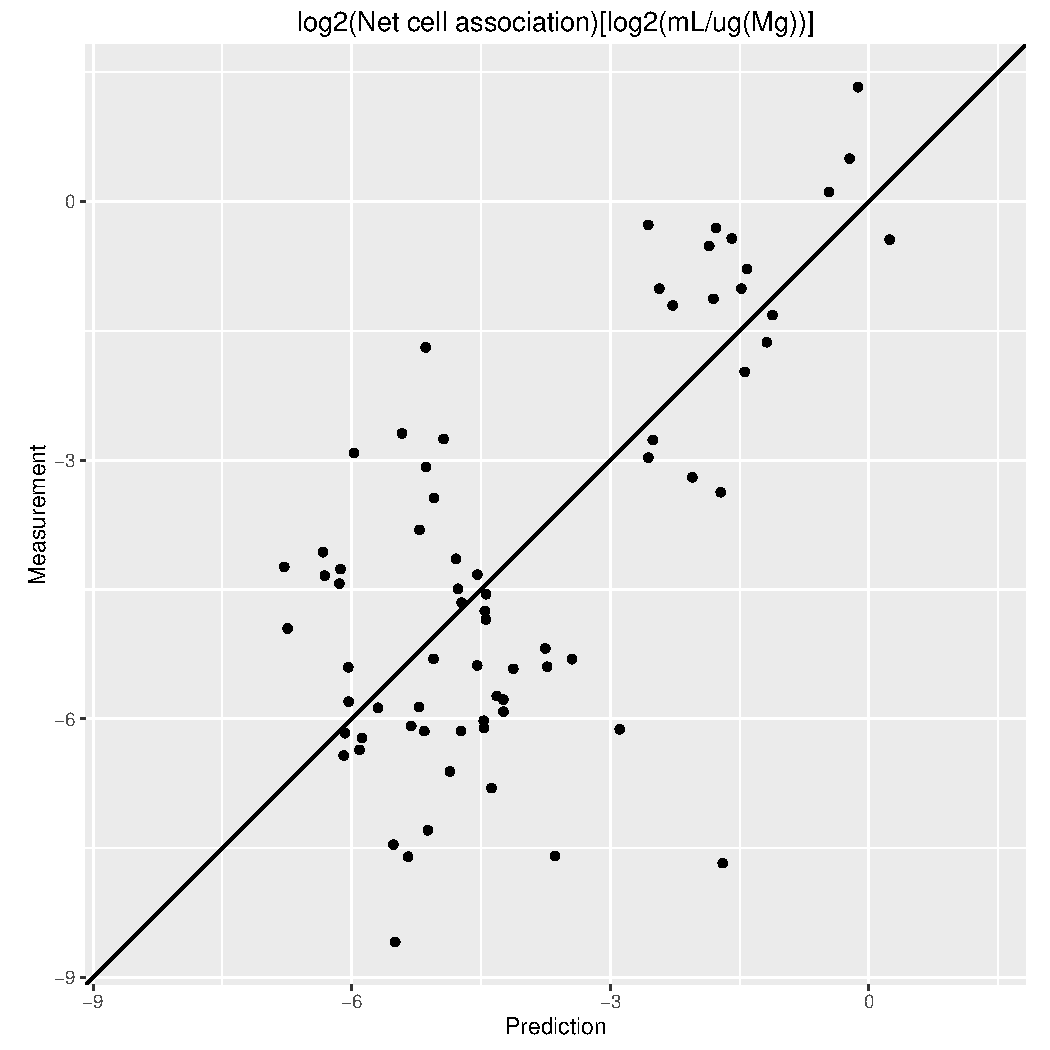
\includegraphics[width=0.3000\textwidth]{figures/MP2D-rf-0.pdf}\label{fig:fingerprint0}
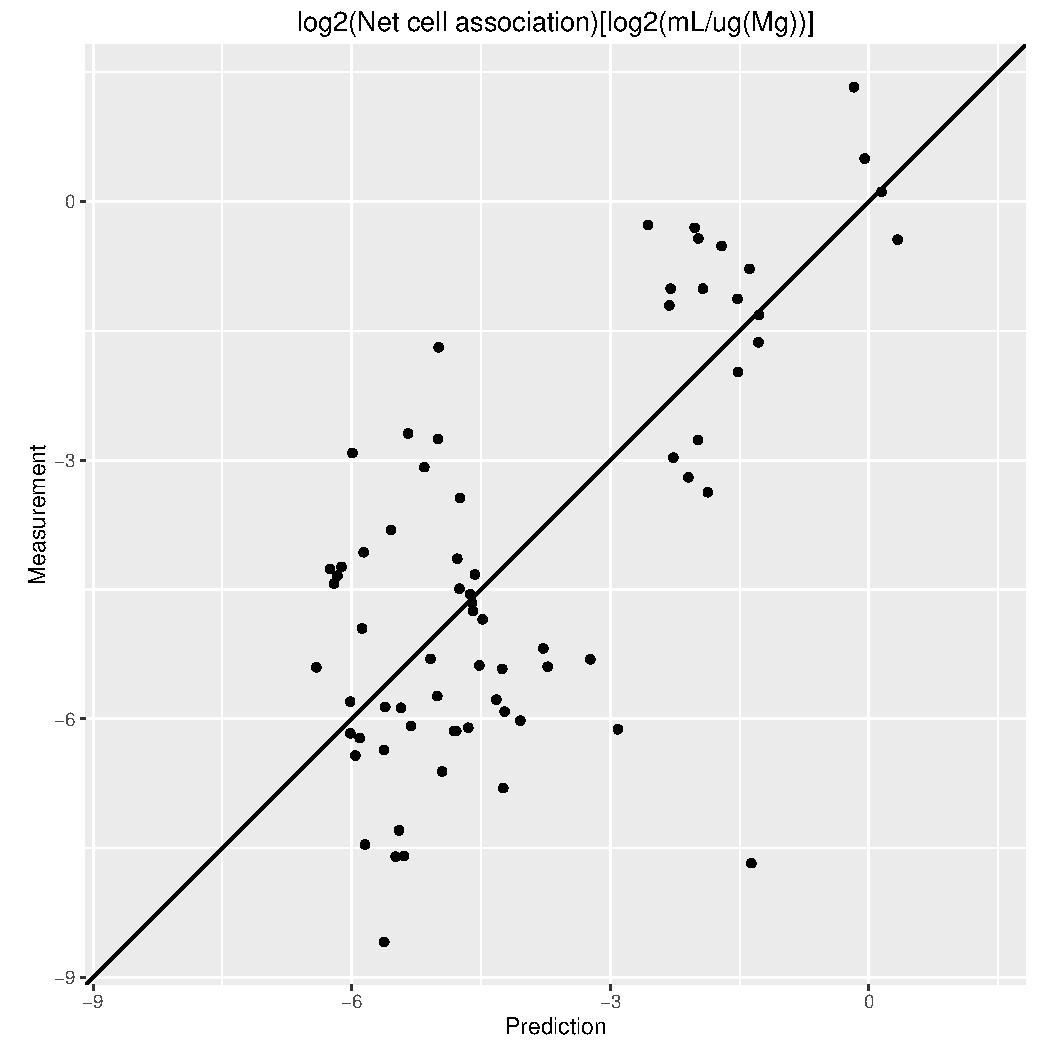
\includegraphics[width=0.3000\textwidth]{figures/MP2D-rf-1.pdf}\label{fig:fingerprint1}
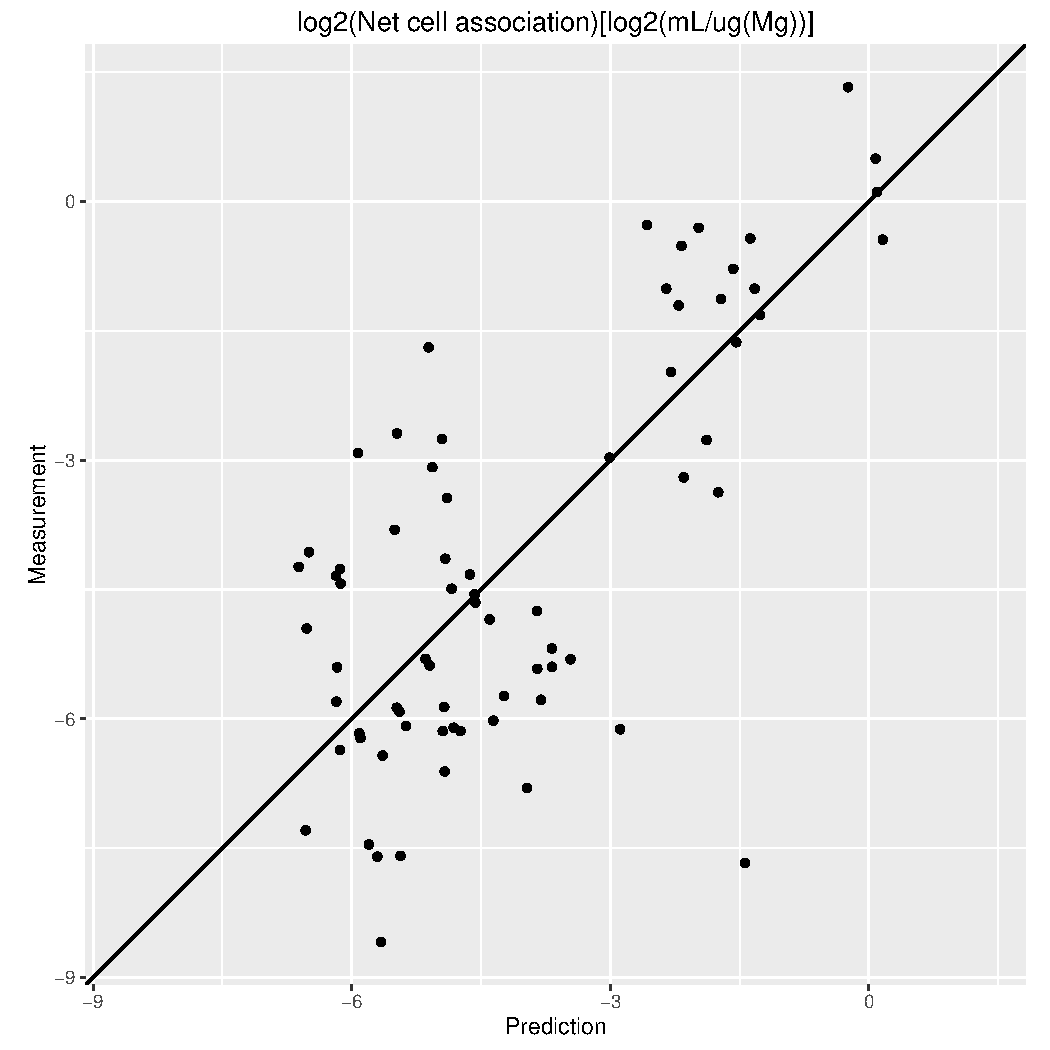
\includegraphics[width=0.3000\textwidth]{figures/MP2D-rf-2.pdf}\label{fig:fingerprint2}
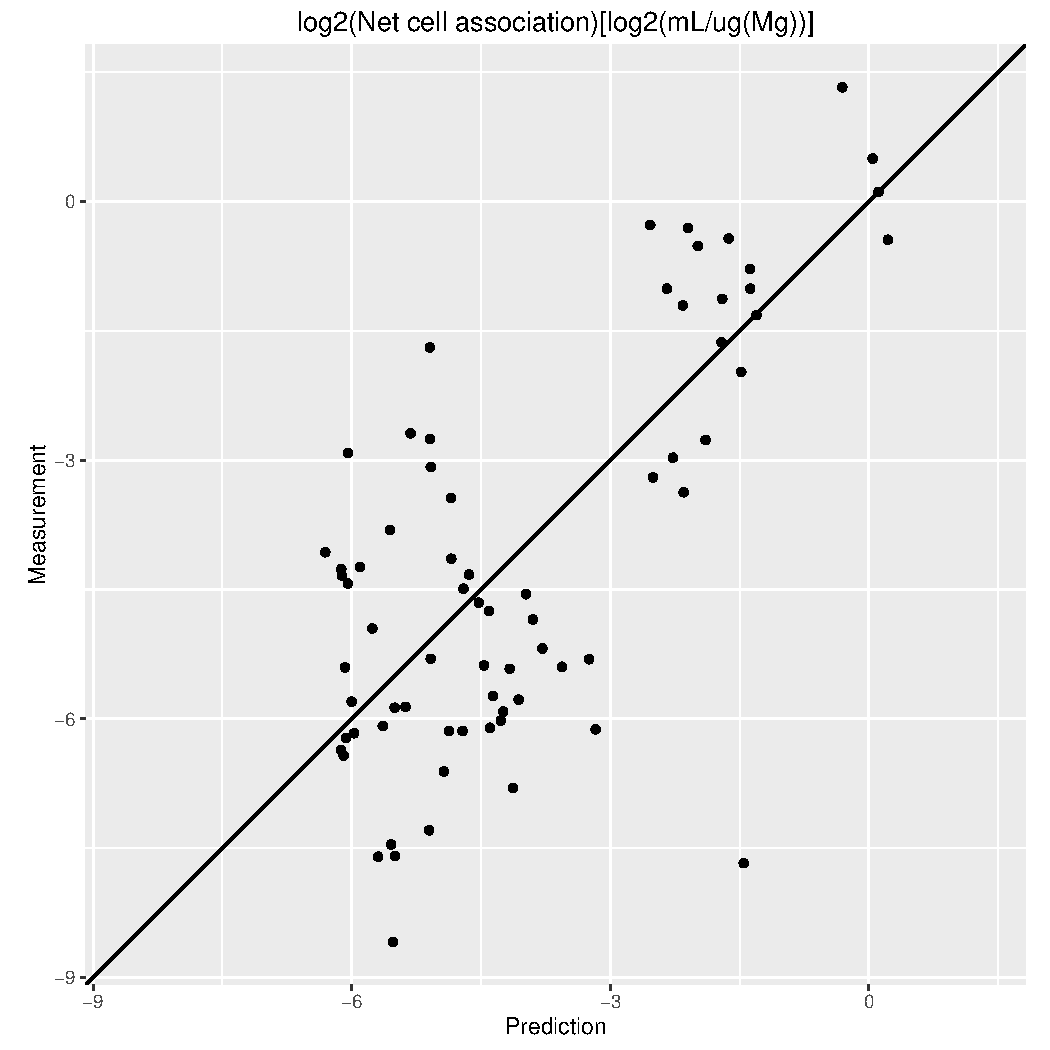
\includegraphics[width=0.3000\textwidth]{figures/MP2D-rf-3.pdf}\label{fig:fingerprint3}
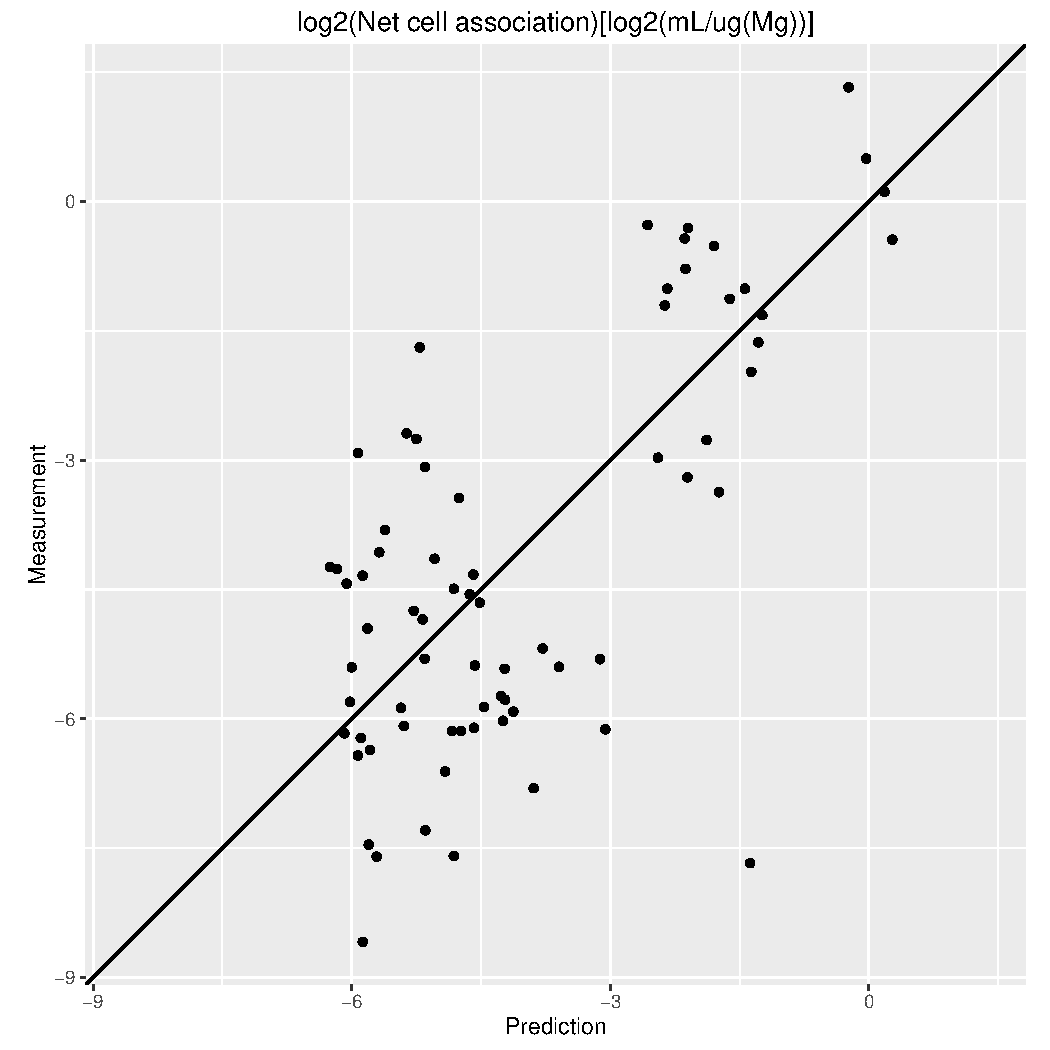
\includegraphics[width=0.3000\textwidth]{figures/MP2D-rf-4.pdf}\label{fig:fingerprint4}

\caption{Correlation of predicted vs.~measured values for five
independent crossvalidations with \emph{MP2D} fingerprint descriptors
and local \emph{random forest} models}

\label{fig:fingerprint}

\end{figure}

\begin{figure}[H]

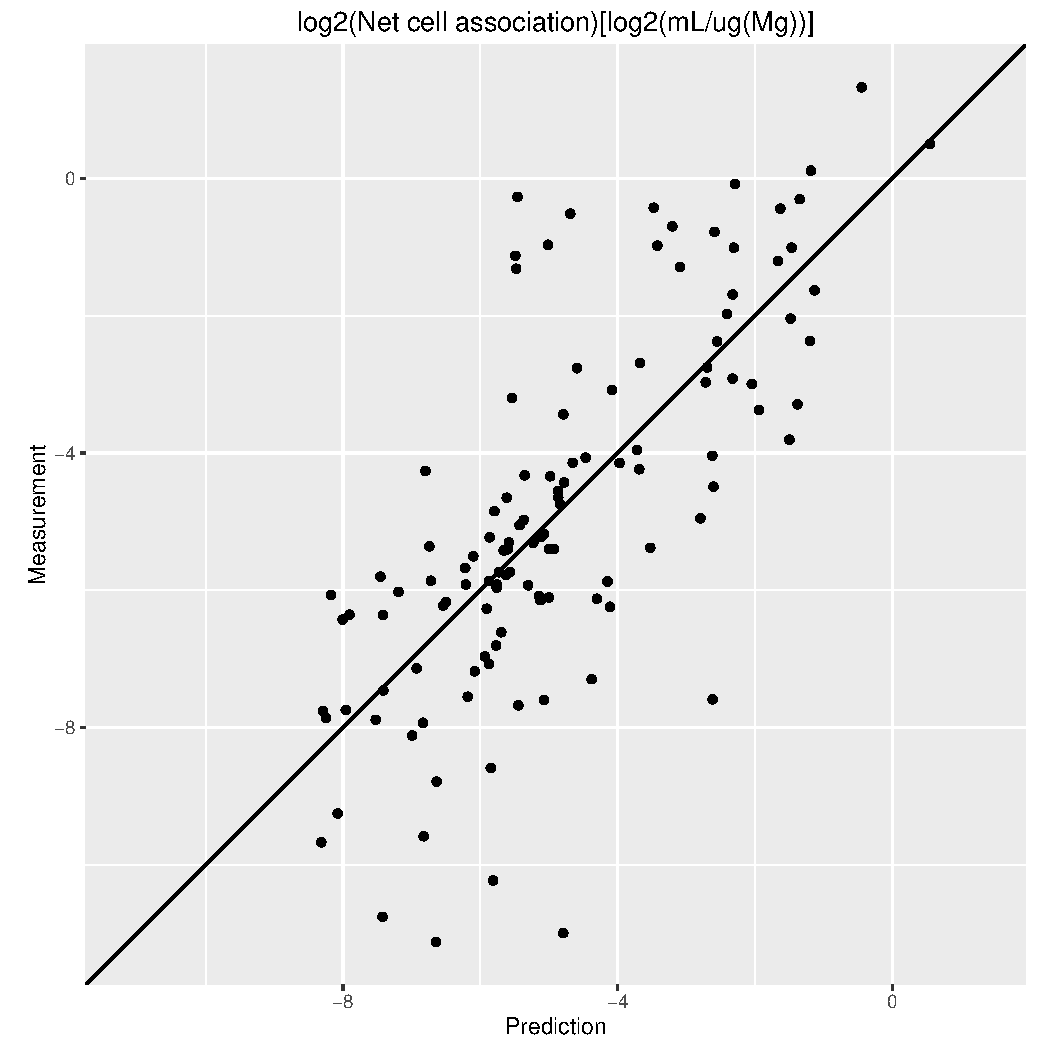
\includegraphics[width=0.3000\textwidth]{figures/PCHEM-rf-0.pdf}\label{fig:pchem0}
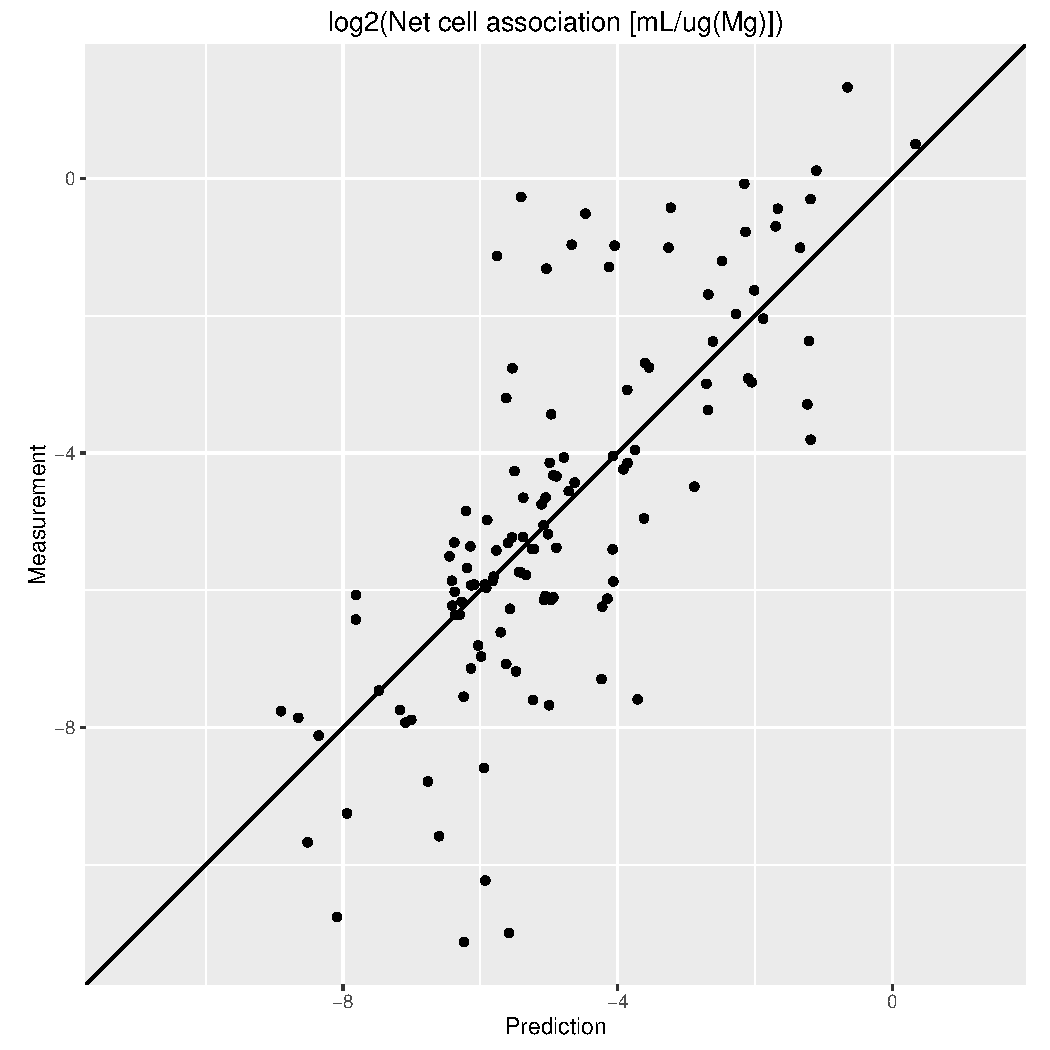
\includegraphics[width=0.3000\textwidth]{figures/PCHEM-rf-1.pdf}\label{fig:pchem1}
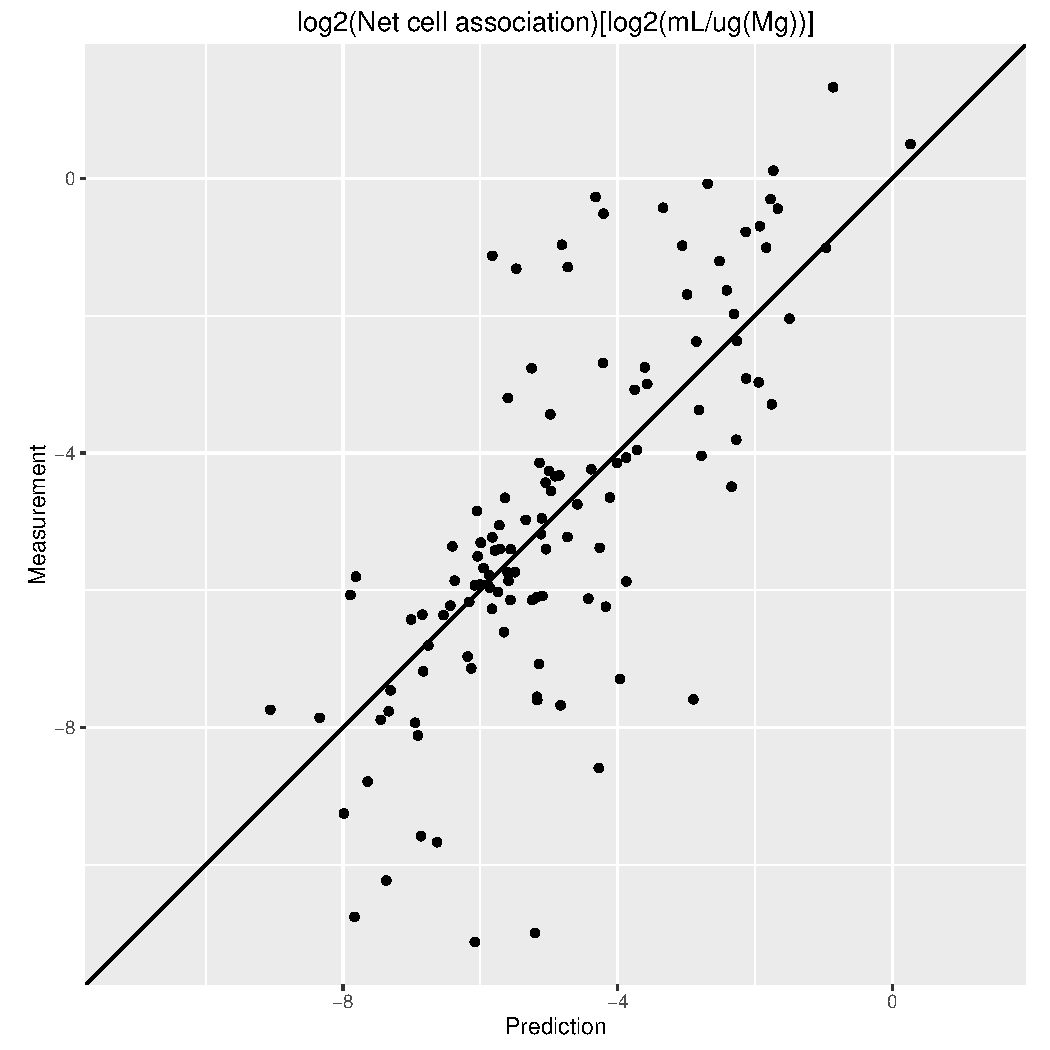
\includegraphics[width=0.3000\textwidth]{figures/PCHEM-rf-2.pdf}\label{fig:pchem2}
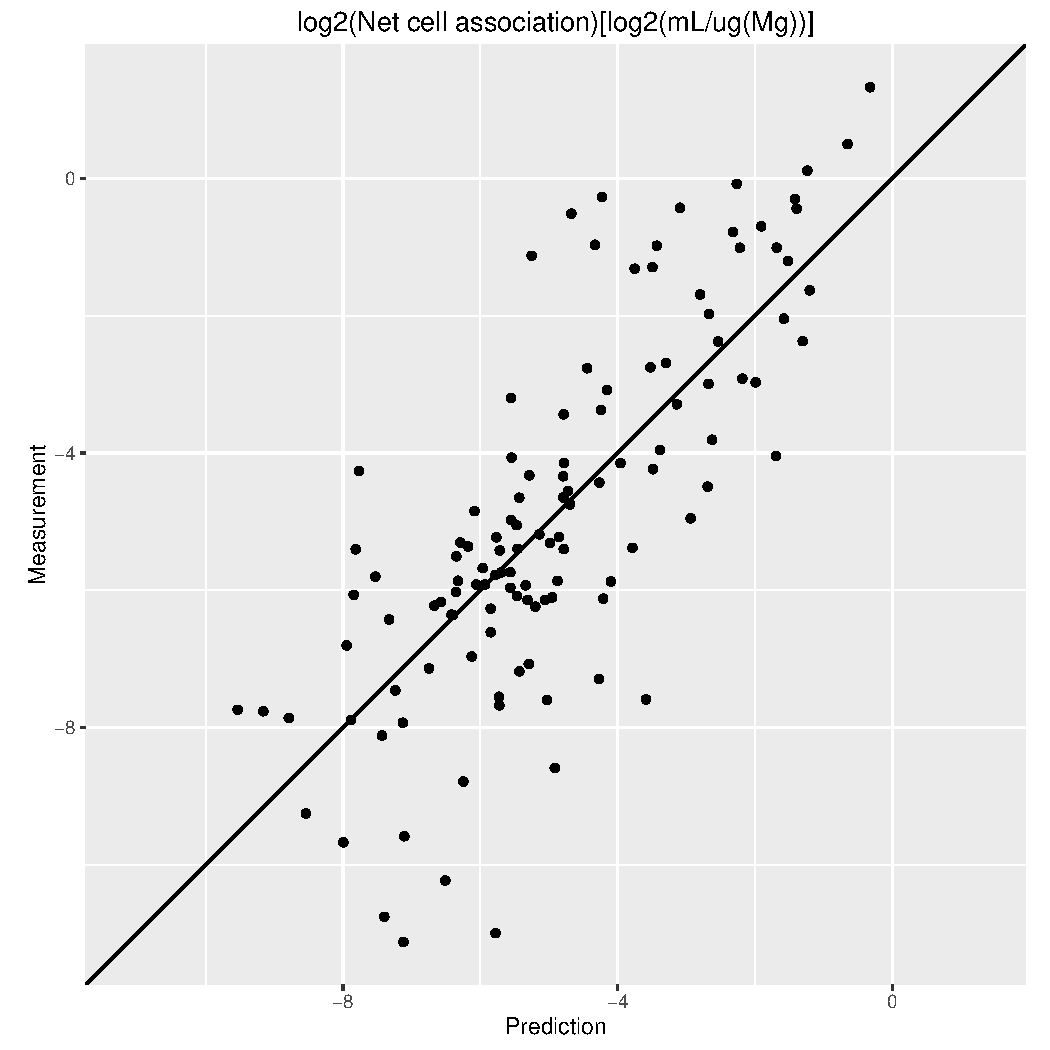
\includegraphics[width=0.3000\textwidth]{figures/PCHEM-rf-3.pdf}\label{fig:pchem3}
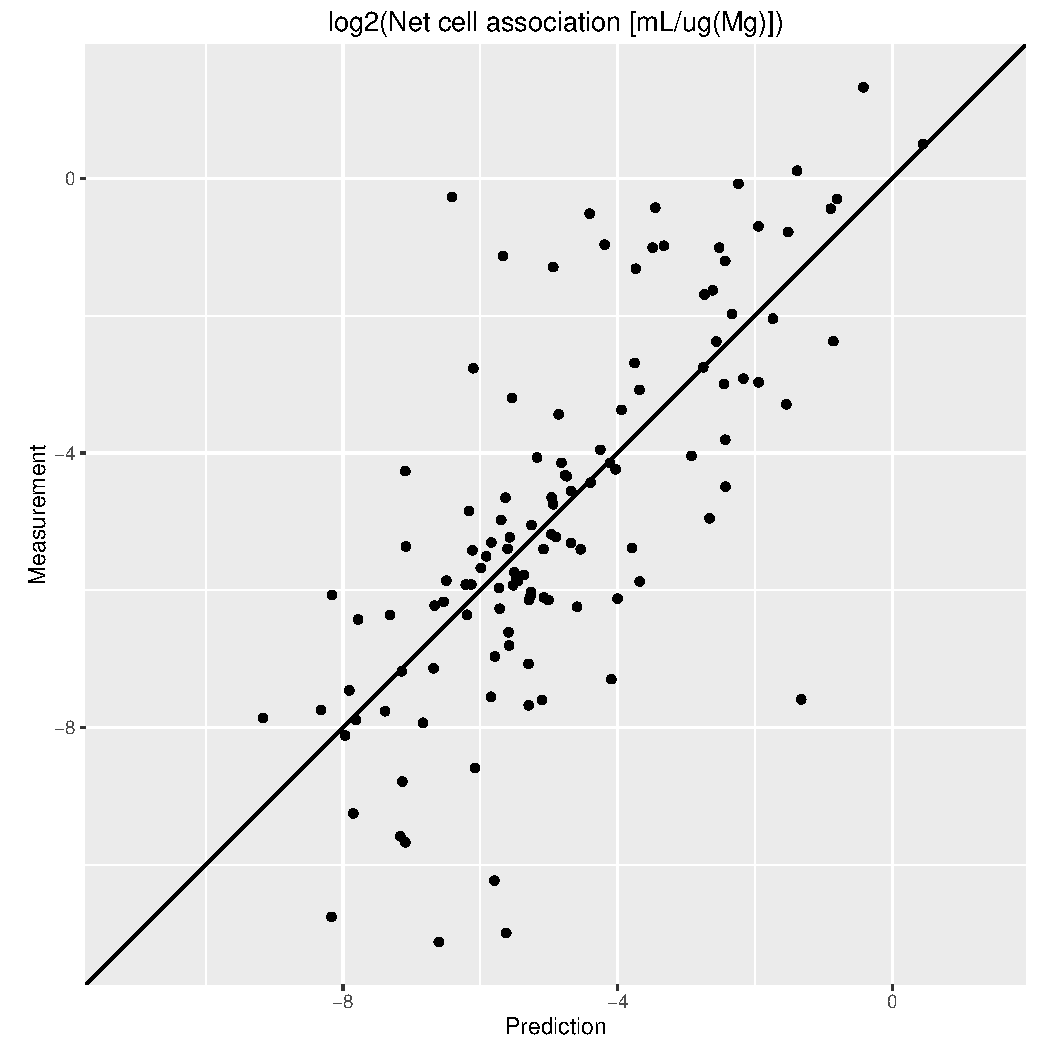
\includegraphics[width=0.3000\textwidth]{figures/PCHEM-rf-4.pdf}\label{fig:pchem4}

\caption{Correlation of predicted vs.~measured values for five
independent crossvalidations with \emph{P-CHEM} descriptors and local
\emph{random forest} models}

\label{fig:pchem}

\end{figure}

\begin{figure}[H]

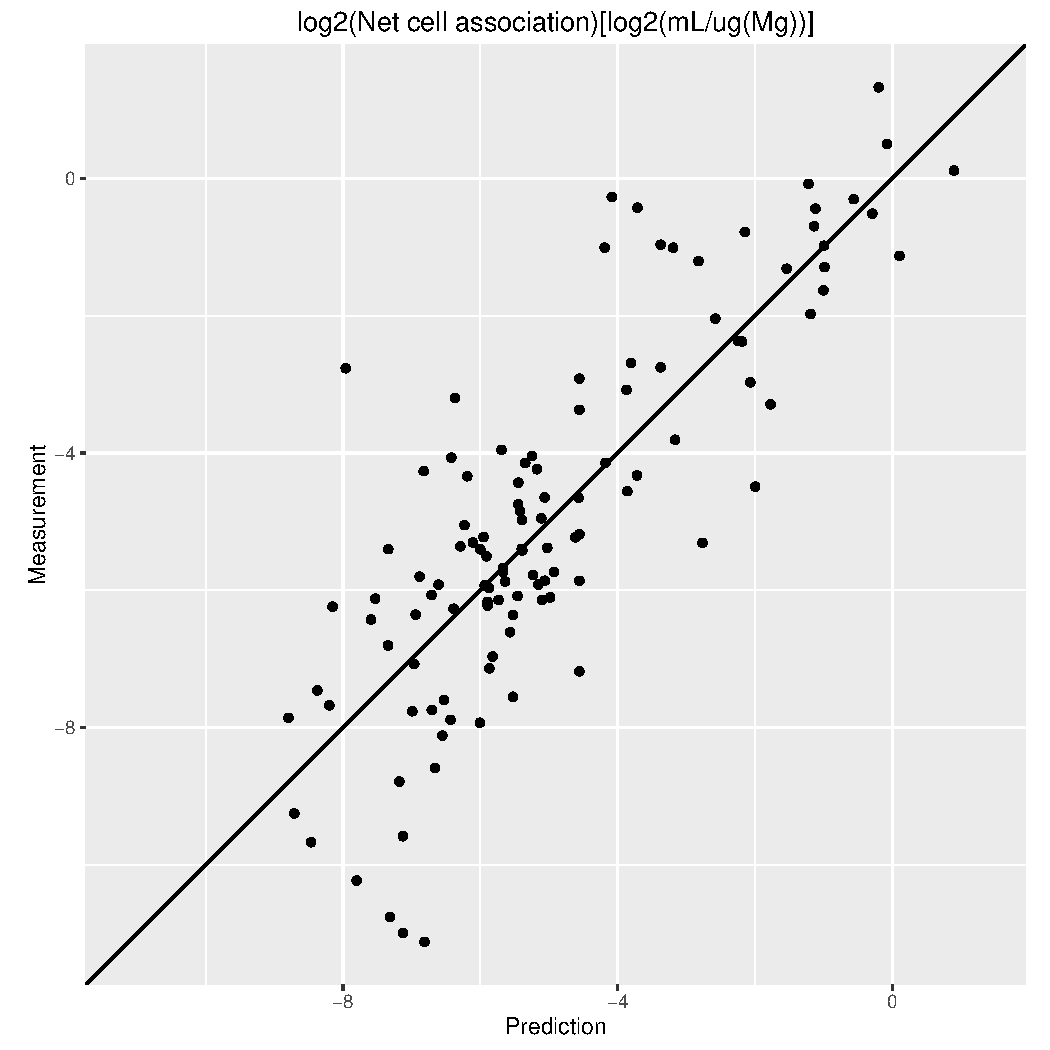
\includegraphics[width=0.3000\textwidth]{figures/Proteomics-rf-0.pdf}\label{fig:prot0}
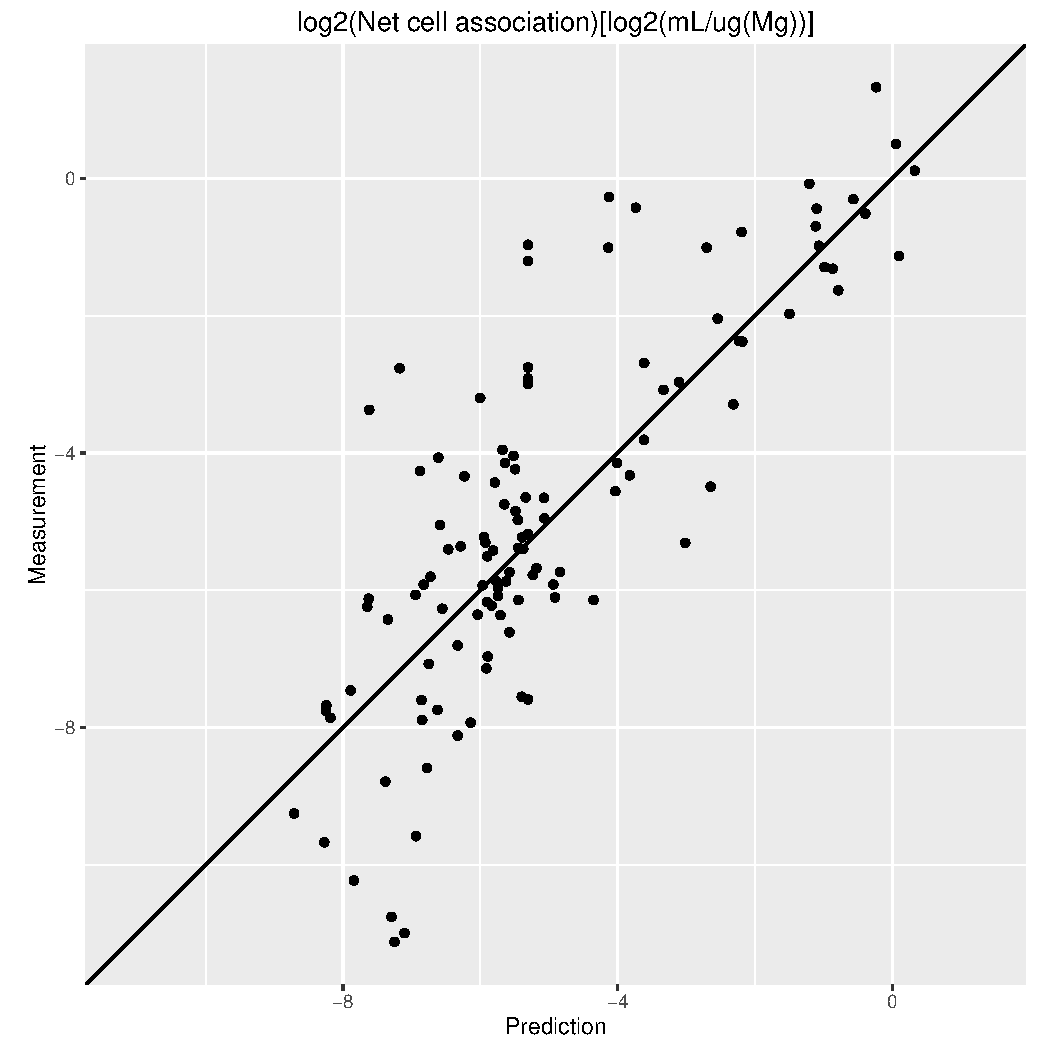
\includegraphics[width=0.3000\textwidth]{figures/Proteomics-rf-1.pdf}\label{fig:prot1}
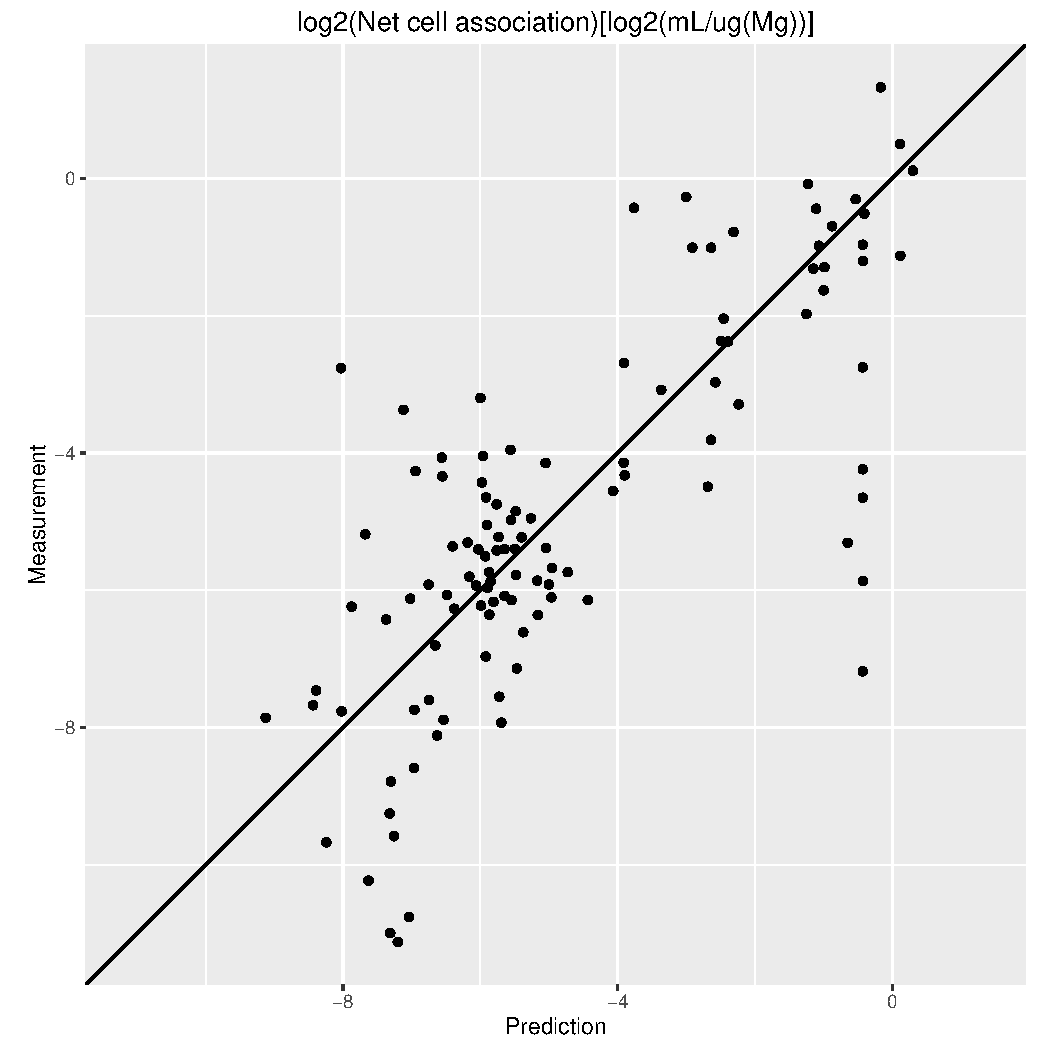
\includegraphics[width=0.3000\textwidth]{figures/Proteomics-rf-2.pdf}\label{fig:prot2}
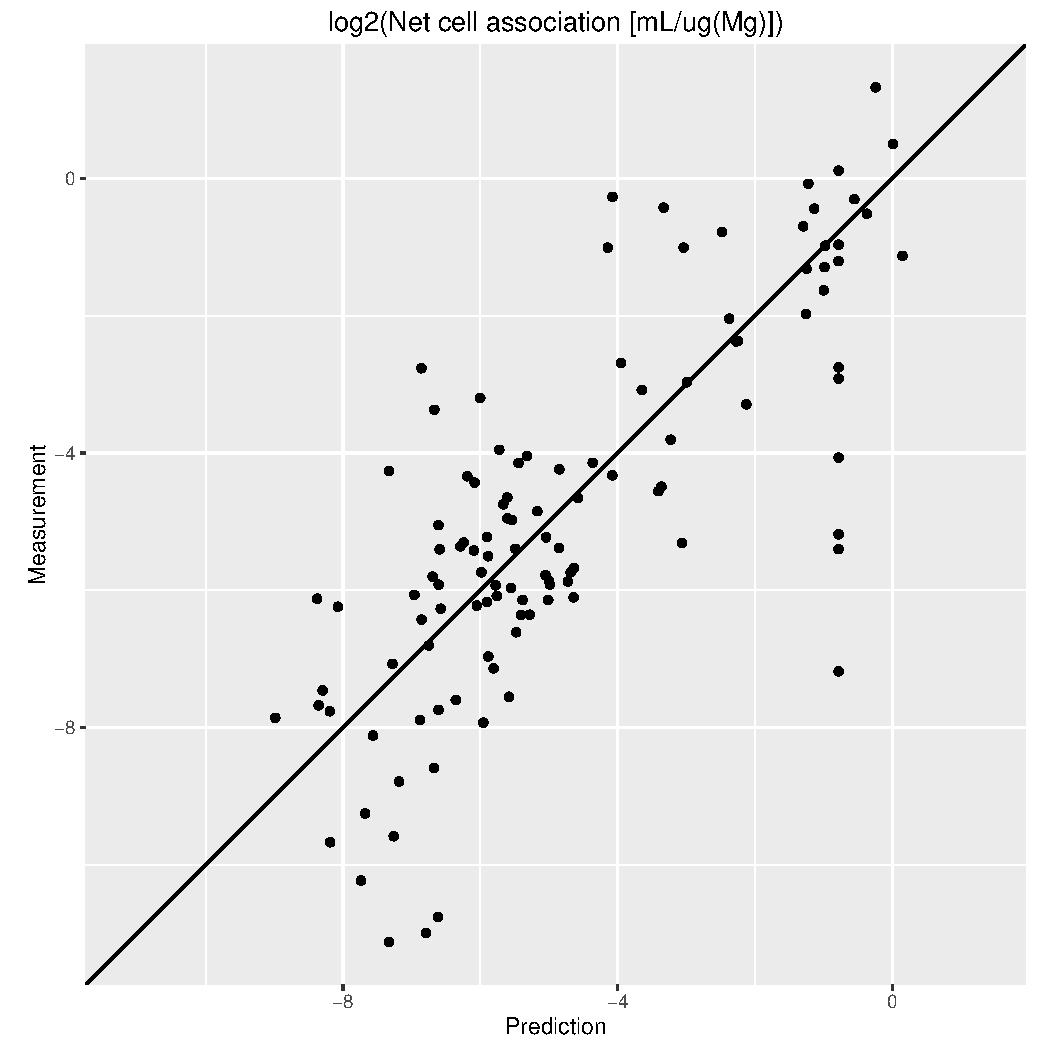
\includegraphics[width=0.3000\textwidth]{figures/Proteomics-rf-3.pdf}\label{fig:prot3}
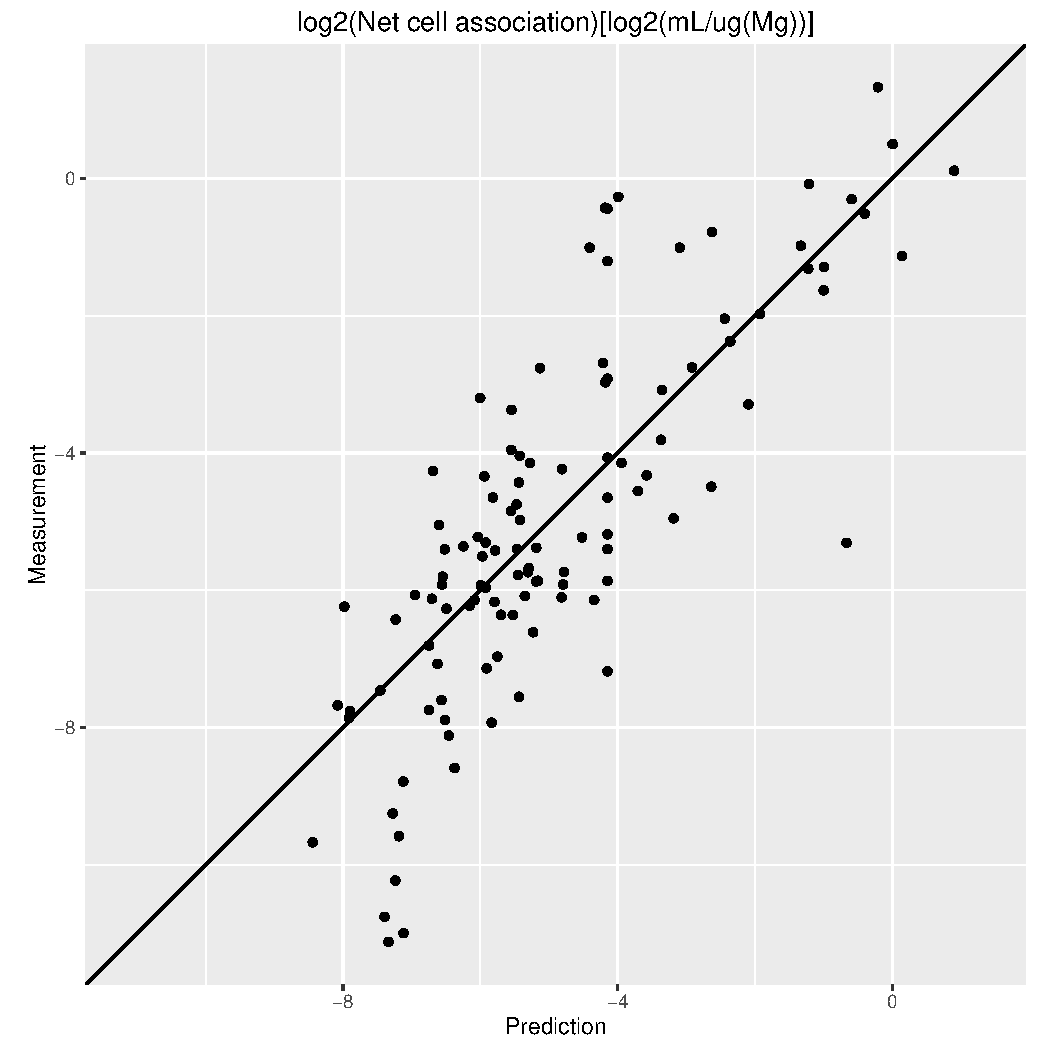
\includegraphics[width=0.3000\textwidth]{figures/Proteomics-rf-4.pdf}\label{fig:prot4}

\caption{Correlation of predicted vs.~measured values for five
independent crossvalidations with \emph{Proteomics} descriptors and
local \emph{random forest} models}

\label{fig:prot}

\end{figure}

\end{document}
